\documentclass[twoside,11pt,preprint]{article}

% Any additional packages needed should be included after jmlr2e.
% Note that jmlr2e.sty includes epsfig, amssymb, natbib and graphicx,
% and defines many common macros, such as 'proof' and 'example'.
%
% It also sets the bibliographystyle to plainnat; for more information on
% natbib citation styles, see the natbib documentation, a copy of which
% is archived at http://www.jmlr.org/format/natbib.pdf

% Available options for package jmlr2e are:
%
%   - abbrvbib : use abbrvnat for the bibliography style
%   - nohyperref : do not load the hyperref package
%   - preprint : remove JMLR specific information from the template,
%         useful for example for posting to preprint servers.
%
% Example of using the package with custom options:
%
% \usepackage[abbrvbib, preprint]{jmlr2e}

\usepackage{jmlr2e}

\usepackage[utf8]{inputenc}
\usepackage[T1]{fontenc}
\usepackage{amsmath}
\usepackage{subfig}
\usepackage{floatrow}
\DeclareMathOperator\logit{logit}
\newcommand{\better}{\succ\,}
\newcommand{\colu}[1]{{\em #1}}
\newfloatcommand{capbtabbox}{table}[][\FBwidth]
\def\tightlist{}
\usepackage{booktabs}
\usepackage{longtable}
\usepackage{array}
\usepackage{multirow}
\usepackage{wrapfig}
\usepackage{float}
\usepackage{colortbl}
\usepackage{pdflscape}
\usepackage{tabu}
\usepackage{threeparttable}
\usepackage{threeparttablex}
\usepackage[normalem]{ulem}
\usepackage{makecell}
\usepackage{xcolor}

% Definitions of handy macros can go here


% Heading arguments are {volume}{year}{pages}{date submitted}{date published}{paper id}{author-full-names}

\jmlrheading{1}{2022}{1-48}{4/00}{10/00}{wainer22a}{Jacques Wainer}

% Short headings should be running head and authors last names

\ShortHeadings{BBT: Comparison of multiple algorithms on multiple data sets}{J. Wainer}
\firstpageno{1}

\begin{document}

\title{A Bayesian Bradley-Terry model to compare multiple ML algorithms on multiple data sets}

\author{\name Jacques Wainer \email \href{mailto:wainer@ic.unicamp.br}{\nolinkurl{wainer@ic.unicamp.br}}\\
       \addr Artificial Intelligence Lab, RECOD.ai\newline Institute of Computing\newline University of Campinas\newline Campinas 13083-970, Brazil.
       }

\editor{}

\maketitle

\begin{abstract}%   <- trailing '%' for backward compatibility of .sty file
This paper proposes a Bayesian model to compare multiple algorithms on multiple data sets, on any metric. The model is based on the Bradley-Terry model, that counts the number of times one algorithm performs better than another on different data sets. Because of its Bayesian foundations, the Bayesian Bradley Terry model (BBT) has different characteristics than frequentist approaches to comparing multiple algorithms on multiple data sets, such as \citet{demsar} tests on mean rank, and \citet{benavoli2016should} multiple pairwise Wilcoxon tests with p-adjustment procedures. In particular, a Bayesian approach allows for more nuanced statements regarding the algorithms beyond claiming that the difference is or it is not statistically significant. Bayesian approaches also allow to define when two algorithms are equivalent for practical purposes, or the region of practical equivalence (ROPE). Different than a Bayesian signed rank comparison procedure proposed by \citet{benavoli2017time}, our approach can define a ROPE for any metric, since it is based on probability statements, and not on differences of that metric.\newline
This paper also proposes a local ROPE concept, that evaluates whether a positive difference between a mean measure across some cross validation to the mean of some other algorithms is should be really seen as the first algorithm being better than the second, based on effect sizes. This local ROPE proposal is independent of a Bayesian use, and can be used in frequentist approaches based on ranks.\newline
A R package and a Python program that implements the BBT is available.
\end{abstract}

\begin{keywords}
  Bayesian,
  Bradley-Terry model,
  Comparison of classifiers,
  Comparison of regressors,
  Multiple data sets,
  Multiple algorithms
\end{keywords}

\hypertarget{introduction}{%
\section{Introduction}\label{introduction}}

Almost any research in Machine Learning that proposes a new model or a
new algorithm it will compare with some previous research, likely on
multiple data sets. Machine learning algorithms are measured using
different metrics; to list a few in classification tasks: accuracy,
Cohen kappa, balanced accuracy, AUC (area under the ROC curve), F1 ,
MCC (Matthew's correlation coefficient), AP (average precision or area
under the PR-curve), g-means, Bier score, and so on. For regression
tasks: RMSE (root mean squared error), MAE (mean absolute error),
\(R^2\) (coefficient of determination) and adjusted \(R^2\), MAPE (mean
absolute percentage error), maximum residual error, etc. There are
other metrics for hierarchical classes \citep{kosmopoulos2015evaluation},
for multi-label problems \citep{6471714} and metrics for NLP generation
\citep{Celikyilmaz20}, multi-objective optimization
\citep{riquelme2015performance}, among a myriad of evaluation metrics for
other different tasks.

It is commonly understood that one should not aggregate measures on
different data sets. That is, it is commonly understood that a 0.76
accuracy in one data set and a 0.96 accuracy in another data set
should not be aggregated together, to compute, for example, the mean
accuracy of 0.86 on the two data sets. The intuition seems to be that
the same gain in accuracy \emph{does not mean the same} on different values
of the base accuracy; an improvement of the accuracy from 76\% to 78\%
is much less ``impressive'' or ``significant'' than a gain from 96\% to
98\%, although in both cases the gain is of 2 percentage points.
Therefore two algorithms, one with with 78\% and 96\% accuracy in both
data sets, and the other with 76\% and 98\%, have the same mean
accuracy, but the second seems ``better'' than the first, since the
second algorithm's gain of 2\% on the second data set is more
``significant'', or more ``impressive'' than its 2\% loss on the first data
set!

However, metrics like accuracy, and AUC, and others, are at least
\textbf{comparable}, in the sense that one can say when one measure in one
data set is better than the measure on another data set. If algorithm
A achieved an AUC of 0.78 in one data set and an AUC of 0.86 on
another data set, one can claim that the second measure (0.85) was
better than the first -- a statement so obvious that it is odd to see it
written down. And if the comparison procedure needs to order the
measures for each algorithm in order to compute the median value or
the mean value (which, as discussed, is not considered a ``correct''
step) one can do it. There are measures, specially in regression
tasks, that are \textbf{not comparable} across different data sets. For
example, is an RMSE of \$30'000,00 on predicting housing values of
Boston suburbs better or worse than a RMSE of 3.3 on predicting the
quality of red wine (a number between 0 and 10)?

The comparable property is important because some comparison
strategies, those based on pairwise Wilcoxon tests \citep{benavoli2017time, benavoli2016should, STAPOR2021107219}, compute for each algorithm
the median of the measures on the different data sets and then compare
these medians, but to compute the median one must have a comparable
metric across different data sets. If the \$30'000,00 and the 3.3 are
RMSE errors from the same algorithm, how would one rank them in order
to compute the median RMSE of this algorithm across the different data
sets?

The goals of a comparison procedure are in order of importance:

\begin{enumerate}
\def\labelenumi{\arabic{enumi}.}
\item
  The procedure should tell which algorithm is better, which is second place, which one
  is third place and so on when measured on a particular set of data
  sets. We will call this the \textbf{aggregated ranking} of the
  algorithms for that set of data sets.
\item
  The procedure should compute how confident or how hopeful one should be that the ordering
  will remain true when one tests the same algorithms on a different
  data set.
\item
  The procedure should state how much one algorithm is
  better than another and specially when one algorithm is not much
  better than another one, that is, when both algorithm have similar
  performances or when they are equivalent.
\item
  The procedure should not require that all algorithms must be evaluated in all data sets.
\end{enumerate}

There are many alternatives to compute the aggregated ranking. The
usual one is to compute each algorithms' rank within each data set: 1
for the best, 2 for the second, and the average rank in case of ties,
and compute the \textbf{mean rank} for each algorithms. The ranking of the
mean ranks is the final aggregated rank. Another alternative, which
has been justified in the literature \citep{benavoli2016should, STAPOR2021107219}, is to compute the median measure
for each algorithm (provided the metric is comparable) and the
aggregated ranking is the rank of the medians. There are also
numerous alternatives for ranking aggregation discussed in other
disciplines: ranking are called preferences in social choice theory
and there is a large set of voting procedures to aggregate preferences
\citep{sep-social-choice}. But the aggregation procedures proposed in
other disciplines usually are not associated with some measure of how
confident one can be that a particular item is really ``better'' than
another one in the aggregated rank.

The second goal (evaluation of how confident one should be about the aggregated ranking)
is needed if only a sample of the relevant the population was
measured and ranked. In case of deciding the winners of an election,
or the winners of a sport championship, one is dealing
with the whole population. There is no concern on whether the senator
who won the seat, or the team that won the championship had a
``statistically significant'' victory. The point of the comparison
procedure is just to compute the aggregated ranking. But when
comparing algorithms for machine learning, one is never interested on
the raw aggregated ranking on the set of data sets used in the
comparison; instead, one is interested on claims that can be made
about future data sets regarding the ranking of the algorithms.

The step of computing the confidence on the aggregated ranking is
usually performed using statistical tests that produce for each pair
of algorithms in the aggregated ranking a binary decision or a
continuous measure on whether one can trust that algorithm A is
better than algorithm B or not, for example. Historically, the more common approach
is the use of a null hypotheses significant tests (NHST), also
called a \textbf{frequentist} approach. Frequentist approaches aim at the
binary decision on whether one should accept or not each pair
comparison. The usual statement ``the difference is
statistically significant'' indicates that one should be confident on
that pair comparison. More recently, there has been a move towards a
\textbf{Bayesian} approach to statistical tests which will not return a binary decision on
accepting or not a pair comparison in the aggregated ranking, but
define a probability that ``A is better than B''.

Regarding the third goal, there is a clear interest in stating that
one algorithm is similar to another for practical purposes. The usual
frequentist methods cannot make this claim\footnote{There are
frequentist tests that determine when two alternatives do not have
practical difference. These are known as equivalence tests [@eqvtest]
but are not of common use in Machine Learning or other areas of
Computing.}; some researchers wrongly assume that if there is no
statistical difference between two algorithms, they are similar or
equivalent. A non significant difference in frequentist test only
indicates that the sample size was not large enough to find the
statistical significance. With a large enough sample size, all
p-values go to 0 \citep{cosma, kruschke2015bayesian} and thus all
differences become significant. On the other hand, Bayesian methods do
allow one to make claims of practical equivalence as we will see
below (section \ref{sec:bayestests}).

Finally, the fourth goal: it is desirable not to require that all algorithms run all
data sets. Algorithms may not converge for some cases, may demand more
memory than it is available, or may exceed the allotted computational
time to perform the tests. In these cases there will be no corresponding
metric for that algorithm for that data set. The comparison procedure
should handle this gracefully. For frequentist approaches, there is
no clear or agreed upon way to deal with missing measures, as we will
discuss below.

This paper proposes a new comparison procedure based on the number of
times an algorithm is better than another on the different data sets. In more details:

\begin{itemize}
\item
  The statistical framework for our proposal is the Bradley-Terry
  model for ranks, which assumes that each item being compared,
  algorithms in this case, has a latent ``merit number'' or ``ability'',
  and that the probability that one item is better than another is a
  function only of the two items' merit numbers.
\item
  The aggregated ranking of the algorithms is the ordering of these merit numbers.
\item
  We propose a Bayesian implementation of the Bradley-Terry model. The Bayesian implementation will allow to compute probabilities that one algorithm is better than another, and that is the measure of one's confidence in the ordering.
\item
  Because we are using a Bayesian model we can define when two
  algorithms are equivalent for practical purposes. In Bayesian
  testing, the range of values for which one claims there is no
  practical differences is called a region of practical equivalence or
  ROPE.
\item
  Our proposal of
  ROPE is in the probability space (a claim on probabilities) and not
  on the metric space (a claim on differences of accuracy or
  differences of RMSE). This allows our notion of ROPE to be generic
  across different metrics, and perfectly understandable (and
  modifiable) by different researchers even in the case they do not
  have experience on comparing algorithms on that particular metric.
\item
  We defined a concept of local ROPE, a decision criteria when
  comparing to algorithms on a particular data set, based on the fold
  data for the two algorithms, that decides whether one algorithm is
  better than another. This decision is not just based on the
  difference between the two mean measures, but takes into
  consideration the ``noise level'' or formally, the effect size of the
  differences.
\end{itemize}

This paper is laid out as follows: Section \ref{sec:tut} is a short
tutorial on frequentist tests for multiple comparisons in general, and
Bayesian tests. A reader that knows the basics of frequentist test can
skip section \ref{sec:tut1}; a reader that understands p-value
adjustments in multiple comparisons can skip Section \ref{sec:tut2}. Section \ref{sec:prev}
discusses the previous frequentist and Bayesian approaches to
comparing multiple algorithms on multiple data sets. Section
\ref{sec:btmod} discusses this proposal, the use of a Bayesian Bradley
Terry model. Section \ref{sec:exp1} shows some first results of using
the BBT model. Section \ref{sec:lrope} discusses our proposal of
considering more than the mean across different cross-validations when
determining if one algorithm is better than the other. Section
\ref{compare-tests} compare the results of the BBT model with the
previous approaches. Section \ref{predictive} discusses the quality of
the BBT model as a predictive estimation of the future behavior of the
algorithms on new data sets. Section \ref{sec:disc} discusses some of
the advantages and shortcomings of the BBT model, and section
\ref{sec:conc} summarizes the main conclusions.

\hypertarget{a-short-tutorial-on-frequentist-and-bayesian-multiple-comparisons}{%
\section{\texorpdfstring{A short tutorial on frequentist and Bayesian multiple comparisons \label{sec:tut}}{A short tutorial on frequentist and Bayesian multiple comparisons }}\label{a-short-tutorial-on-frequentist-and-bayesian-multiple-comparisons}}

Let us assume that different algorithms tested on multiple data sets
are measured using some metric for which calculating the average is an
acceptable procedure (which is not the usual case in Machine Learning
results, as discussed above), and let us also assume that many data sets
were used in the comparison. These two assumptions are necessary for
this tutorial so: a) we can use a \textbf{parametric} frequentist test to
discover which algorithms are significantly different from each other
and b) use a \textbf{Gaussian} based Bayesian modeling of the problem.

\hypertarget{general-aspects-of-frequentist-approach}{%
\subsection{\texorpdfstring{General aspects of frequentist approach \label{sec:tut1}}{General aspects of frequentist approach }}\label{general-aspects-of-frequentist-approach}}

The frequentist approaches, also known as \textbf{NHST} or null hypothesis
statistical testing, will select a few statements of the form ``the
mean of results for algorithm A is different than the mean of results
for algorithm B'', or more succinctly that ``algorithm A is different
than algorithm B'' and claim that \emph{they are true} (but not in these
terms), and for the other possible statements, it will claim that it
cannot decide whether the statement is true or not true. More
formally, NHST will indicate that a difference between two
algorithms or groups is true by the statement ``the difference between algorithm
A and B is \emph{statistically significant}''. The test will indicate that a
difference cannot be shown to be true or false by the statement ``the
difference between algorithms A and B is \emph{not} statistically
significant''.

Internally, most frequentist test models the problem by assuming that
there is no difference between the populations that \emph{generated} the
samples, and compute an approximation of the probability that the
unique source of data for all groups would generate (by chance)
samples that have mean values as different, or more different, than the ones
encountered in the real data. This approximation of the probability
is called \textbf{p-value} and the standard in Machine Learning and most other Science areas is
is that if \(\mbox{p-value} \le 0.05\) then one claims that
the null hypothesis (that all data came from a single population) is
false. Therefore, that the ``differences between the algorithms are real''.

For a statistical test, a \textbf{type 1} error is the
test claiming that the difference between two sets of measures is
``real'' (or more precisely, the test claims that there is enough
evidence to state that there is a difference) when the difference is
not real - a false positive error. A \textbf{type 2} error is the test
claiming that the difference is not real when ``it really is'' - a false
negative error.

Usually, the probability of a type 1 error, that is,
the probability of a false positive error, or the probability of
making a false positive claim is denoted by \(\alpha\). In the Sciences, one is very concern that
false claims will not be made, and thus one sets \(\alpha\) to 0.05 or
lower, which is the threshold of 0.05 for the p-value. The number
\(1-\alpha\) is called the \textbf{significance}, and a frequentist test
which uses \(\mbox{p-value} \le 0.05\) will state that the difference between groups A and B is
statistically significant with 95\% significance. The probability of
a type 2 error is denoted by \(\beta\) - the probability of a false
negative error, or the probability of missing a true claim. The number
\(1-\beta\) is called \textbf{power} of a test. There is no generally
scientific standards for power although some textbooks when teaching
experiment planning or experimental design mention that one should aim at a power of 80\%.

\hypertarget{frequentist-test---anova-plus-post-hoc-tests}{%
\subsection{\texorpdfstring{Frequentist test - ANOVA plus post-hoc tests \label{sec:tut2}}{Frequentist test - ANOVA plus post-hoc tests }}\label{frequentist-test---anova-plus-post-hoc-tests}}

When comparing the mean of multiple groups, the standards frequentist
approach is to perform an \textbf{omnibus} test first, followed, if needed,
by some \textbf{post hoc} tests. The omnibus test assumes as null
hypothesis that all groups came from the same population or
distribution. If the p-value of this test is low enough, then the
conclusion is that not all groups came from the same population, but
this does not tell us which groups are different from each other. This
will be the role of the post-hoc tests. In parametric multiple
comparison procedures, the omnibus test is called ANOVA (Analysis of
Variance) or repeated measures ANOVA, depending on whether the data is
not-paired or paired respectively.

\textbf{Paired} data refer to situations where there is a correspondence
among each data items in each of the groups. For example, each
algorithm was tested on the same set of data sets, and thus one can
make the correspondence of that result in each algorithm to one
particular data set. Usually, in machine learning, one deals with
paired data, but that is not necessary. The alternative to paired data
is called \emph{independent} samples, or \emph{non-paired} data\footnote{In
older statistical texts, or texts used for other scientific areas, the
paired situation is also called *within-subjects*, while the non-paired
is called *between-subjects*.}. Statistical tests differ for paired and
non-paired data, but one can always use a non-paired test on paired
data, but usually with some decrease in power - some differences that
would be significant with the paired test may not be so using the
non-paired test.

Once the comparison passes the omnibus test, one performs the post-hoc
test, which verifies which of the claims ``group A is different than
group B'' has sufficient evidence. There are different ways of
classifying post-hoc tests, but for the purpose of this paper, the
post-hoc test may compute a single critical difference, for example
Tukey's range test. If the difference between two group means is
larger than this critical difference, then one can claim that the
difference between the two groups is statistically significant,
otherwise, the difference is not statistically significant. The
alternative for critical difference post-hoc tests is to compute pairwise p-values, that
is, to compute a separate p-value for each pair of groups. In the
case of multiple p-values, the post hoc test must also adjust each of
the p-values, using some (statistical) \textbf{multiple comparison} or
\textbf{p-value adjustment} procedure.

Statistical multiple comparison procedures is a complex topic in
frequentist statistics \citep{feise2002multiple, rothman1990no, bender2001adjusting}. We refer the reader to
\citep{farcomeni2008review, garcia2008extension} for a deeper
understanding of the issue and the techniques.
But in general terms, let us assume that each pairwise test uses the 0.05
threshold for p-value (this is called the
comparison-wise or individual error rate). If one makes \(k\)
\emph{independent} tests, and summarizes them into a single statement
``\(T_1\) and \(T_2\) and \(T_3\) and \(\ldots T_k\)'' the probability that any
one of the sub-statement (\(T_i\)) is correct is \(1-0.05\). If we assume
that the tests are independent, the probability that all
sub-statements are correct is \((1-0.05)^k\), and therefore, the
probability that the statement as a whole is false is \(1- (1-0.05)^k\).
This is called the family-wise error rate (FWER). If there are 100
tests, the FWER is 0.994, instead of the 0.05 one would expect from
each of the individual tests! If one wants the family-wise error to
be 0.05 one must use a much smaller individual error rate. On first
approximation, if the individual error rate is \(\alpha\), and if one wants the FWER to be 0.05, then:

\begin{align*}
1- (1-\alpha)^k  = 0.05\\
1 - (1^k -k 1^{k-1} \alpha + O(\alpha^2)) = 0.05\\
k \alpha = 0.05 - O(\alpha^2))\\
\alpha = \frac{0.05}{k}
\end{align*}

The calculations above reflects what is known as the Bonferroni test or Bonferroni
correction. The term \(O(\alpha^2)\) indicates that there is a term
with \(\alpha^2\), another with \(\alpha^3\) and so
on. Since \(\alpha\) is small, this calculation assumes that the
\(O(\alpha^2)\) term is very small and does not change the results in
any important way. Therefore, to maintain a FWER of 0.05, when
\(k=100\) each individual test should be accepted if its p-value is less
than 0.0005, that is \(0.05/100\). Statistical multiple test procedures
are usually expressed in terms of adjusting or modifying the original
p-values from each individual test so that one will still use the usual
0.05 threshold. In the example above, the Bonferroni procedure would
multiply each of the original p-values by 100 (limiting the product to
1.00 since p-value is probability), and if any of the adjusted p-value
is lower than 0.05 then one accepts that comparison as statistically
significant.

There are problems with the assumptions for the Bonferroni correction:

\begin{itemize}
\item
  Not all tests are independent especially if one is comparing \(n\)
  different algorithms (or any items). In this case the \(k\) are all
  pairwise comparisons, that is \(k = \frac{n(n-1)}{2}\). If one test
  determines that algorithm A is better than B and B is better then
  C, then the third test, which compares A and C is fully
  determined, and it is not independent of the others. If, on the
  other hand, a test determines that A is better than B and C, the
  third test which compares B and C is indeed independent of the
  other two.
\item
  Not all \(k\) tests will return that a particular
  comparison/difference is statistically significant. If, in the
  last example, the third test determines that there is not enough
  evidence to claim that B is better than C, the final claim will be
  ``A is better than B and A is better than C''. In this case, only
  the result of two tests were incorporated into the final claim.
\end{itemize}

The effective \(k\) one should use in the Bonferroni correction is lower
than the total number of tests and therefore the threshold p-value is
lower ``than it should be.'' This increases the type 2 error of the
procedure - some statements will not achieve the low p-value required
by the Bonferroni correction, but would have low enough p-value if the
correct \(k\) was used.

Beyond the Bonferroni procedure, there are dozen of different p-value
adjustment procedures, among them, Holm, Hochberg, Hommel, Benjamini and
Hochberg, and Benjamini and Yekutieli \citep{padj}. There is no clear
guidelines to select one or other p-adjustment procedures, but all are
more powerful than Bonferroni.

Because of the dependence on the number of comparisons, frequentist
approaches make a distinction between two goals of a
multiple comparisons. The first, and probably more common case, which
is called \textbf{comparisons against a control}, is the situation that
a research proposed a new algorithm and the researcher wants to
compare that algorithm, known as \emph{the control}, against others which are
considered as competitors. The goal of the comparisons is to show
that the control is better or worse than each of its competitors; and
the internal order among the competitors is not needed, nor it is
reported. The second goal, called \textbf{all pairwise
comparisons}, reflects a case where the researcher wants to rank a
set of algorithms on multiple data sets and all pair comparisons
are of interest and are reported. When one is comparing a set of
algorithms against a control, much less comparisons must be made,
which will require a less severe adjustment of the p-values.

\hypertarget{bayesian-tests}{%
\subsection{\texorpdfstring{Bayesian tests \label{sec:bayestests}}{Bayesian tests }}\label{bayesian-tests}}

All Bayesian tests (also known as \textbf{Bayesian estimation procedures})
compute the posterior join distribution of some parameters of the model
that are important for the analysis. The simpler case to discuss is a
Bayesian version of the two samples (non paired) t-test for the means.
A simple Bayesian test will model each set of data (X and Y) as being
samples from two Gaussian distributions with mean \(\mu_X\) and \(\mu_Y\)
and with standard deviation \(\sigma_X\) and \(\sigma_Y\) respectively.
The model also defines that \(\mu_X\) and \(\mu_Y\) are themselves sampled
from another Gaussian with mean \(\mu\) and standard deviation \(\sigma\),
and that \(\sigma_X\) and \(\sigma_Y\) are sampled from a uniform
distribution between \(L\) and \(H\). A more complex model of the same
problem was proposed by \citet{kruschke2013bayesian}. This is expressed by
the following notation:

\begin{align}
x_i & \sim \mbox{Normal}(\mu_X, \sigma_X) \nonumber\\
y_i & \sim \mbox{Normal} (\mu_Y, \sigma_Y)\nonumber\\
\mu_X & \sim \mbox{Normal} (\mu,\sigma) \nonumber\\
\mu_Y & \sim \mbox{Normal} (\mu,\sigma) \label{eq:mod2}\\
\sigma_X & \sim \mbox{Unif}(L,H)\nonumber\\
\sigma_Y & \sim \mbox{Unif}(L,H) \nonumber 
\end{align}

The variables of interests are called \textbf{parameters} and in this case
are \(\mu_X\) and \(\mu_Y\) (and maybe \(\sigma_X\) and \(\sigma_Y\)).

The distributions \(\mbox{Normal} (\mu,\sigma)\) and \(\mbox{Unif}(L,H)\)
are sometimes called \textbf{hyper-priors}. The \textbf{hyper-parameters} \(\mu, \sigma, L\), and \(H\) are set externally so that the distributions for
the true data X and Y are likely. For example, if the measured
average of the data in X is 5 and the measured average of the data in
Y is 5.2, then the random variables \(\mu_X\) and \(\mu_Y\) should be
around 5, and thus the mean of the Gaussian from which both \(\mu_X\)
and \(\mu_Y\) are sampled should have mean (the \(\mu\) hyper-parameter)
of 5.

The width of the hyper-priors, the hyper-parameters \(\sigma\), \(L\),
and \(H\), and even the hyper-prior distributions themselves, are
constraints on the possible values of the parameters. If these
distributions are too narrow, the parameters will likely remain around
a limited range of possible values, and the result of the Bayesian
estimation may be due more to these constraints than the data itself,
which is undesirable. If these hyper-parameters are too large, they may
impose little or too little constraints on the parameters and may have
impacts on the convergence of the MCMC algorithm. A broader version of this
discussion is named the non-informative vs weakly informative vs
strongly informative priors \citep{lemoine2019moving, gelman2017prior}.

In general terms, a Bayesian test will compute (or sample, as we will
see below) the posterior distribution of the parameters of interests,
in this case \(\mu_X\) and \(\mu_Y\) given the data. That is, we want to
compute:

\[ P(\mu_X,\mu_Y | M, X, Y) = K \; \:  P(X,Y| M, \mu_X, \mu_y) P(\mu_X, \mu_Y | M)\]

where \(X\) and \(Y\) are the data, and \(M\) is the model itself
(equations \ref{eq:mod2}), and \(K\) is a constant that normalizes the
distribution \(P(\mu_X,\mu_Y| ...)\) so it adds to 1 (or whose integral
is 1). Given the distribution \(P(\mu_X,\mu_Y | M, X, Y)\) one can
compute, for example, \(P( \mu_X > \mu_Y | M, X, Y)\), that is, the
probability that the mean of the Gaussian distribution that
\emph{generated} X (Gaussian distribution from which X was sampled) is
larger than the mean of the distribution that generated Y. If
probability is 0.8, then the researchers are 80\% sure that X comes
from a population whose mean is greater than the population from which Y
comes from, and they can report that. This claim is different than the
claim that researchers using a frequentist approach can make.

\hypertarget{rope}{%
\subsubsection{ROPE}\label{rope}}

Another useful statement to derive from the posterior distribution is
the probability that the difference between \(\mu_X\) and \(\mu_Y\) is of
no practical consequence. If \(\delta\) is the value below which the
difference is of no practical consequence, then the value of
\(P(|mu_X - mu_Y| < \delta | M, X, Y)\) is the probability that there is
no important difference between \(\mu_X\) and \(\mu_Y\). The value
\(\delta\) in Bayesian analysis is called \textbf{region of practical
equivalence} or \textbf{ROPE}. Differences smaller than the ROPE are
considered as differences that do not matter for practical purposes.

\hypertarget{mcmc-and-convergence}{%
\subsubsection{MCMC and convergence}\label{mcmc-and-convergence}}

Usually, Bayesian tests do not compute the probability distribution
\(P(\mu_X,\mu_Y | M, X, Y)\) analytically, but use some instance of the
MCMC family of algorithms to sample tuples \(\langle {\mu_X}_j,{\mu_Y}_j \rangle\) from that distribution, indicated as
\(\langle {\mu_X}_j,{\mu_Y}_j \rangle \sim P(\mu_X,\mu_Y | M, X, Y)\).
In the case of a sample set of \(\langle {\mu_X}_j,{\mu_Y}_j \rangle\),
computing the probability that \(\mu_X > \mu_Y\) is just counting the
proportion of the samples for which \({\mu_X}_j > {\mu_Y}_j\).

MCMC algorithms will converge on the limit to
the target distribution, but in practice the MCMC algorithm will run
for a pre-determined number of steps, and the convergence diagnostics
allow the user to assess whether the samples returned are ``good
samples'' from the target distribution. We refer the reader to
\citet{mcmcdiag} for a comprehensive discussion on convergence diagnostics.

Convergence diagnostics are necessary every time one runs a Bayesian
model. The diagnostic informs users that the set of tuples they
receive from the algorithm are indeed samples of the posterior
distribution of the parameters or that the user may need to run more
steps of the MCMC algorithm, or even redefine their Bayesian model.

\hypertarget{posterior-predictive-check}{%
\subsubsection{Posterior Predictive Check}\label{posterior-predictive-check}}

\emph{Posterior predictive} diagnostics attempts to measures how well
the Bayesian model (in our case the model proposed in Equation
\ref{eq:mod1}) models the data itself.

If the MCMC converges, it will
correctly return tuples sampled from the posterior distributions of
the parameters, but if the model itself does not correctly describe
the data, the posterior distributions of the parameters will be less
useful than expected.

The goal of the posterior predictive check (PPC) is to verify that the
data generated by the model (given the posterior values of the
parameters) is similar to the observed data. In other words, when the
parameters assume the ``correct values'' (the posterior distribution of
the parameters), one can ``run the model forward'', in the case above
compute a new value of \(x_{ik}\).\footnote{This statement is a
simplification in order to provide the reader with an intuitive
understanding of the process. Formally, the same MCMC algorithm also
samples from $ P(X_{rep}, Y_{rep} | M, X, Y)$ where $X_{rep}$ is the
data generated from the model ($M$) given the real data ($X$ and
$Y$).} The distribution of, for example \(x_{1k}\), that is, all the
generated data for the first \(x\) data should be compared with ``the
real data'' \(x_1\). If the model is appropriate to the problem, the
real data should be very similar to the set of generated data.

There are other forms of evaluating how well a model fits the data
based on approximations of the leave-one-out cross validation, among them, WAIC
(Watanabe-Akaike information criteria) \citep{watanabe2010asymptotic} and
loo \citep{vehtari2017practical}. We will not go into details regarding
these approaches but we will notice they are useful when comparing
different models among themselves. We will use them further below
when discussing alternative modeling.

\hypertarget{bayesian-tests-for-multiple-comparisons}{%
\subsubsection{Bayesian tests for multiple comparisons}\label{bayesian-tests-for-multiple-comparisons}}

We have discusses above a particular Bayesian model to compare \textbf{two}
sets of data. If one performs all pairwise comparisons using some
frequentist test, that would require using some p-adjustment
procedure. But it is yet unclear whether there is or not a problem in
performing multiple Bayesian comparisons. It has been claimed that if
the Bayesian model is hierarchical/multilevel there is no problem in
performing multiple comparisons \citep{gelman2012we}. Hierarchical models
are similar to the line \ref{eq:mod2} in the Bayesian model described
above where the two parameters are sampled from a single distribution.
In a hierarchical model with multiple comparisons, one would need an
equation like \ref{eq:mod2} for each of the parameters of interest
\(\mu_X, \mu_Y, \mu_W, \ldots \mu_Z\), all sampled from the \emph{same}
distribution. This will pool the different estimates of \(\mu_i\)
towards each other, what is called \emph{partial pooling} or \emph{shrinkage}.
One such hierarchical model is the Bayesian ANOVA \citep[ch.~19]{kruschke2014doing}.

\hypertarget{frequentist-versus-bayesian-approaches}{%
\subsection{Frequentist versus Bayesian approaches}\label{frequentist-versus-bayesian-approaches}}

There are many differences between frequentist and Bayesian
approaches. We will not discuss them in this paper, but we point the
reader to \citet{benavoli2017time} discussion on the limitations of the
frequentist approach.

\hypertarget{previous-frequentist-and-bayesian-approaches}{%
\section{\texorpdfstring{Previous Frequentist and Bayesian approaches \label{sec:prev}}{Previous Frequentist and Bayesian approaches }}\label{previous-frequentist-and-bayesian-approaches}}

In this section we will discuss the previous approaches to comparing multiple algorithms on multiple data sets.

\hypertarget{demsars-procedure-mean-rank-plus-nemenyi-test-and-extensions}{%
\subsection{\texorpdfstring{Demsar's procedure (mean rank plus Nemenyi test) and extensions \label{sec:demsar}}{Demsar's procedure (mean rank plus Nemenyi test) and extensions }}\label{demsars-procedure-mean-rank-plus-nemenyi-test-and-extensions}}

The most standard frequentist procedure for comparison of multiple
algorithms on multiple data sets is the one defined by \citet{demsar}. The
main steps of this comparison procedure are:

\begin{itemize}
\tightlist
\item
  each data set results are converted to ranks, 1 for the best
  result, 2 for the second best results;
\item
  ties are treated as average rank. If two algorithms have the same
  measure on a data set and they are the fourth best ranked
  algorithms for a data set, then the two algorithms receive the
  rank of 4.5, the average of 4 and 5, and the next algorithm receives rank 6;
\item
  the final order is the decreasing order of the mean rank across
  all data sets. That is, an algorithm with a lower mean rank is
  \emph{better} than an algorithm with a higher mean rank;
\item
  the degree of confidence in this order is given by a pairwise
  binary statement on whether one should be confident or not that
  the algorithm \(i\) is better than algorithm \(j\). The statement that
  one should be confident on each pair comparison is indicated by
  the usual phrase in NHST
  that ``the difference \emph{is} statistically significant'';
\item
  the computation of the pair comparisons significance is
  accomplished by first applying the Friedman test (the omnibus test) and then applying the Nemenyi
  test which returns a critical difference on the mean rank; if
  the difference on the mean ranks of two algorithms is smaller than
  the critical difference, then the difference between the two
  algorithms is \emph{not} statistically significant.
\end{itemize}

\citet{demsar} also
discusses a different comparison procedure when comparing against a
control.

\citet{garcia2008extension} proposed and tested different extensions to
Demsar's procedure. The extensions use different post-hoc procedures:
Shaffer's static and Bergmann-Hommel's procedures. The authors claim
that these post-hoc procedure are stronger than
the Nemenyi test. \citet{garcia2010advanced} also proposed new omnibus
tests, the Friedman aligned ranks and Quade tests, and tested other
post-hoc procedures for p-value adjustments, and concluded that the
procedures Holm, Hochberg, Hommel, Holland and Rom produce equivalent
results.

\citet{demsar} and extensions can be summarised as a family of \emph{non-parametric} and \emph{paired} multiple procedures computed using the rank of the algorithms within each data set. The omnibus procedure is Friedman \citep{demsar} or others \citep{garcia2010advanced}, and the post-hoc procedures can be based on critical difference on the ranks \citep{demsar, garcia2008extension} or can be even Wilcoxon pairwise procedures on the rank data followed by the many alternative p-adjustment procedures \citep{garcia2010advanced}.

\hypertarget{pairwise-wilcoxon-plus-p-value-adjustment-procedures}{%
\subsection{\texorpdfstring{Pairwise Wilcoxon plus p-value adjustment procedures \label{sec:pairwil}}{Pairwise Wilcoxon plus p-value adjustment procedures }}\label{pairwise-wilcoxon-plus-p-value-adjustment-procedures}}

\citet{benavoli2016should} discuss that comparison procedures based on mean
ranks have a problem: if the comparison of the algorithms A, B, C, D,
and E yield that the differences between A and B are significant,
changing the other algorithms to say F, G, and H may result in a
non-significant difference between A and B. That is, the result of
the comparison of two algorithms depend on the other ones being
compared. They suggest using a pairwise Wilcoxon signed rank test
between the metrics obtained by each algorithms for all data sets,
followed by an appropriate multiple comparisons adjustment procedure.
This procedure is also suggested by \citet{STAPOR2021107219}.

Of relevance for this paper is that this approach will not create an
aggregated ranking based on the mean rank of each algorithm across the
data sets, but an aggregated ranking based on the median measure of
each algorithm across the data sets. Of course, such procedure
require comparable metrics. The distinction between comparing against
a control and all pairwise comparison is trivially implemented in this
approach.

Before we advance to Bayesian approaches, let us discuss the issues
regarding missing data in the frequentist approaches discussed so
far - the cases where an algorithm did not run for some data set. The
problem is that there is no standard way of dealing with the missing
data. For mean rank approaches such as Demsar's procedure one could
not compute the rank for the algorithm that did not run for a
particular data set, and not use this missing rank when computing the
mean rank, but that would imply that not running on a data set would
attribute to that algorithm its mean rank. This is possible but it is
not standard. For example \citet{fernandez2014we} did something similar but
that procedure was criticised by \citet{wainberg2016random} as adding a
positive bias to the algorithm that did not run on the data set. One could do the same
for the pairwise Wilcoxon tests, but again that would mean that an
algorithm that did not run on a data set receives its median measure
for that data set. We do not have an opinion on whether this is the
correct thing to do, or if one should assign to the algorithm the
worst rank; the problem is that there is no agreed upon way of dealing
with missing data for frequentist tests.

\hypertarget{bayesian-pairwise-signed-rank-test}{%
\subsection{\texorpdfstring{Bayesian pairwise signed-rank test \label{sec:bsr}}{Bayesian pairwise signed-rank test }}\label{bayesian-pairwise-signed-rank-test}}

\citet{benavoli2017time} developed two forms of a Bayesian version of the
Wilcoxon signed rank test (BSR), and argued for their use within the
Machine Learning practice. The first form uses a single measure per
algorithm and per data set, usually the mean of different measures
using some form of cross-validation, a standard approach in
Machine Learning. The second, more complex, form (called Bayesian
hierarchical correlated t-test further expanded in \citet{corani2017statistical}) uses each measure from each of the
cross-validations (which we will call a \emph{fold} below regardless if
k-fold is being used as the cross validation procedure) into the
computation, but they suggest that practitioners should use the
simpler form.

The model's parameter is the mean of the pairwise difference between
of the accuracy of the algorithms on the different data sets, and the model
computes a distribution of probability for this parameter. The authors state
that if this parameter is between -0.01 and 0.01 (or a ROPE of 1\%)
there is no practical difference between the two algorithms being
compared. The justification for the 1\% ROPE \emph{for accuracy} is not
presented in the paper, but that number is not too different than the
ROPE threshold proposed by \citet{wainer2016}, but in this case based on some
empirical evidence, and twice as large than the one proposed by
\citet{WAINER2021115222}, based on different set of empirical evidence.

On the data level, as we discussed above, a 1\% of difference may or
may not be important, depending on the accuracy itself. A 1\% change for a
79\% accuracy is likely insignificant but a 1\% change for an accuracy
of 98\% is impressive. Given the range of accuracy values that appear
in practical cases of comparing two classifiers (some high, some low)
the authors are claiming that changes on the \emph{mean value} of less than
1\% are irrelevant from a practical point of view.

Even if one accepts the 0.01 ROPE for accuracy, there is no agreed
upon, or even proposed (as far as this author is aware) ROPEs for AUC,
F1, MCC, and other classification metrics and for comparable
regression metrics. And, of course, there will be no ROPE for
incomparable metrics, nor will the Bayesian signed rank method be
applicable to incomparable metrics, given that the mean of the
pairwise differences is not conceptually well defined (what is the
mean of a difference of \$7400,00 and a difference of 1.3 points in the
RMSE of two algorithms?).

The Bayesian signed rank test was defined for comparing \emph{two}
algorithms on multiple data sets, and thus there may be problems in
applying it to multiple comparisons. \citet{benavoli2017time} do not perform
any multiple comparison in the paper. They do perform many
signed-rank procedures with different algorithms but not with the goal
of ranking those algorithms. At the end of the paper, they
acknowledge that the Bayesian signed rank model does not have an
hierarchical component that would allow its unproblematic use in
multiple comparisons. But they use an argument put forth by
\citet{kruschke2013bayesian} that the use of ROPE would mitigate the false
alarm rate (making false positive claims). This is not a fully
accepted argument, and even if it is correct, that would \emph{require} the
use of ROPE in any comparison. Since \citet{benavoli2017time} only proposes
a ROPE for accuracy, unless other proposals for ROPEs for other
metrics are advanced, using BSR for other metrics would be imprudent.

\hypertarget{bradley-terry-model}{%
\section{\texorpdfstring{Bradley-Terry model \label{sec:btmod}}{Bradley-Terry model }}\label{bradley-terry-model}}

The Bradley-Terry (BT) model \citep{bradley1952rank} is mainly used to rank
``players'' in ``tournaments'' where the payers compete pairwise in
matches, for example, soccer teams or chess payers. The BT model
attributes to each player \(X_i\) an \emph{intrinsic value} or \emph{ability}
\(w_i\). The intrinsic value relates to the probability that player \(i\)
will win player \(j\) in a match by:

\[ P(X_i \mbox{ wins } X_j) = P(X_i \succ\,X_j) = \frac{w_i}{w_i + w_j} \]

The final ranking of the players is defined by the rank of their
intrinsic values \(w_i\). We will use the notation \(i \succ\,j\) to
indicate that \(X_i \mbox{ wins } X_j\). In Machine Learning ``wining'' depends on the metric. If the metric is accuracy
or AUC, the highest value wins; if the metric is RMSE or other error
metrics, or execution time, or energy consumption, the lower value wins.

The intrinsic values are invariant to a multiplicative constant, that
is, if the set \(\{w_i\}\) correctly models all the probabilities \(P(a \succ\,b)\), so will \(\{\alpha w_i\}\). Therefore, to specify a single
set of intrinsic values, one also requires that \(\sum w_i = 1\).

An alternative to the \(w_i\) is to use their natural logarithms \(\beta_i = \log w_i\).
The useful formula regarding \(\beta\) is:

\begin{equation*}
\mbox{logit}(i \succ\,j) = \log \frac{P(i \succ\,j)}{1-P(i \succ\,j)} = \log \frac{P(i \succ\,j)}{P(j \succ\,i)} = \beta_i - \beta_j 
\end{equation*}

The \(\beta\) values are invariant to additive constant, since the \(w_i\)
were invariant to multiplicative constants. The usual way to specify a
single set of solutions is to require that \(\sum \beta_i = 0\).

The standard BT model does not deal with ties and thus \(1 - P(i \succ\,j) = P(j \succ\,i)\), but there are some extensions of the BT
model that incorporate ties into the model \citep{rao1967ties, davidson1970extending, baker2021modifying}. We will discuss the model proposed by \citet{davidson1970extending} in Section \ref{test-ties}. One common practice
is to keep the standard BT model without ties but to change the data
provided to the estimation procedure so that a tie between \(i\) and \(j\)
is modeled a counting as both a victory for \(i\) and for \(j\) or sometimes
as half a victory for each. We will elaborate this point further
in Section \ref{test-ties}.

\hypertarget{mle-and-bayesian-estimation-of-the-w-or-beta}{%
\subsubsection{\texorpdfstring{MLE and Bayesian estimation of the \(w\) or \(\beta\) \label{sec:bayesbt}}{MLE and Bayesian estimation of the w or \textbackslash beta }}\label{mle-and-bayesian-estimation-of-the-w-or-beta}}

Let us assume that players \(i\) and \(j\) play \(N_{ij}= N_{ji}\) matches against each other,
and \(W_{ij}\) is the number of matches that \(i\) wins and \(W_{ji}\) is
the number of matches \(j\) wins (and thus \(N_{ij} = W_{ij} + W_{ji}\)
given that there are no ties). If we assume that \(W_{ii} = 0\), and if
there are \(t\) players, then the likelihood function is:

\[L(w) = \prod_{i,j=1}^t (\frac{w_i}{w_i+w_j } )^{W_{ij} }\]

Given all the \(W_{ij}\), the maximum likelihood (MLE) estimation is the set \(w^* = \{w_1, w_2, \ldots w_n \}\) such that

\[w^* = \mbox{argmax}_w L(w)\]

There has been proposals for different algorithms to compute the MLE
(and MAP) solutions for the BT model
\citep{hunter2004mm, caron2012efficient}. Some research refer to the
case where the comparison graph is sparse \citep{li2021, butler2004},
which is not the case in our problem -- we assume that most of the
algorithms will be compared to almost all other algorithms on most
data sets.

The Bayesian model for BT is based on the beta coefficients:

\begin{align} 
 W_{ij} &\sim \mbox{Binomial}(N_{ij}, \frac{e^{\beta_i}}{e^{\beta_i} +  e^{\beta_j}}) \label{eq:mod1} \\
 \beta_i &\sim \mbox{Normal}(0,\sigma) \nonumber \\
 \sigma &\sim \mbox{LogNormal}(0,0.5) \nonumber
\end{align}

The binomial expression captures the fact that the number of times \(i\)
wins from \(j\) is a binomial distribution given the total number of
matches between \(i\) and \(j\) (\(N_{ij}\)) and the probability that \(i\)
will win each match (\(P(i \succ\,j) = \frac{w_i}{w_i+ w_j})\).

The \(\beta\) parameters can have positive and negative values and thus
it is reasonable to sample them from a normal distribution with mean
0, and variance \(\sigma\) (a hyper-parameter). This is the
hierarchical component of the Bayesian BT model (BBT): all \(\beta_i\)
are sampled from the same distribution and thus the model can be used
to compare multiple algorithms, since there will be partial pooling.
The hyper-prior for \(\sigma\) is a log-normal distribution, as proposed
by \citet{btstan}, but in section \ref{test-hyper} we explore other
hyper-priors and show that there is no difference on whether one uses
them.

\hypertarget{exploration-of-the-bbt}{%
\section{\texorpdfstring{Exploration of the BBT \label{sec:exp1}}{Exploration of the BBT }}\label{exploration-of-the-bbt}}

This section will explore some results of using the BBT model on a
particular set of algorithms and data sets (Section
\ref{sec:data}). We will present some of the outputs of the model
(Section \ref{sec:out1}) We also discuss two forms of diagnostics
check (Sections \ref{sec:conv1} and \ref{sec:ppc1}), and a concept of
ROPE appropriate for the model (Section \ref{sec:rope}). We finalize
with a discussion on the two interpretation of the basic parameters of
the model (Section \ref{strong-weak}) and a discussion on comparison
against a control algorithm (Section \ref{sec:control}).

\hypertarget{data}{%
\subsection{\texorpdfstring{Data \label{sec:data}}{Data }}\label{data}}

We will explore the use of the BBT model on four use-cases regarding
the comparison of machine learning algorithms on multiple data sets.
The details of how the data was obtained are not relevant for this
paper, but for the sake of completeness we will briefly describe it.
The four use cases are called small-small, small-large, medium-medium,
and large-large.

The large-large (\emph{ll}) use-case is the results of running 16 out of
the box classifiers (without tuning their hyper-parameters) on 132
data sets. The classifiers are listed and briefly described
below. The data sets are the first 132 smallest data sets from the set
curated by \citet{Olson2017PMLB}. We use the accuracy metric so we can compare the results with the BSR procedure.

The first set of 13 algorithms are implementations of classification
algorithms available in the scikit-learn package \citep{scikit-learn}
(version 1.1.1), which also defines their particular set of default
values for the hyper-parameters (not listed here).

\begin{itemize}
\tightlist
\item
  \emph{dt}: Decision tree
\item
  \emph{gbm}: Gradient boosting classifier,
\item
  \emph{knn}: K-nearest neighbors
\item
  \emph{lda}: Linear discriminant analysis,
\item
  \emph{lr}: Logistic regression
\item
  \emph{mlp}: Multi-layer perceptron
\item
  \emph{nb}: Naive Bayes Gaussian classifier
\item
  \emph{passive}: Passive-aggressive classifier,
\item
  \emph{qda}: Quadratic discriminant analysis,
\item
  \emph{rf}: Random forest
\item
  \emph{ridge}: Ridge regression
\item
  \emph{svm}: SVM with a RBF kernel
\item
  \emph{svml}: SVM with linear kernel
\end{itemize}

The next set of two algorithms are implemented in the XGBoost package \citep{Chen:2016:XST:2939672.2939785} (version 1.6.1):

\begin{itemize}
\tightlist
\item
  \emph{xgb}: Gradient boosting classifier as implemented by the XGBoost package
\item
  \emph{xrf}: Random forest as implemented by the XGBoost package
\end{itemize}

And the final algorithm is from the LightGBM package \citep{ke2017lightgbm} :

\begin{itemize}
\tightlist
\item
  \emph{lgbm}: Gradient boosting classifier as implemented by the LightGBM
\end{itemize}

The large-large results reflect the case were a large number of
algorithm is being compared on a large number of data sets. Most of
the curated sets of data sets, for example PMLB \citep{Olson2017PMLB}, the
KEEL imbalance data sets \citep{alcala2011keel}, the OpenML-CC18 Curated
Classification benchmark \citep{oml-benchmarking-suites} include on the
order of 100 data sets. We believe that, in a large case, a
researcher will be comparing around 20 different algorithms, but we
are aware of some published research that test many more algorithms,
for example around 50 \citep{wainer2021tune}, or around 100
\citep{fernandez2014we, wang2021comparing}. But it is important to notice
that these three examples did not perform statistical tests to confirm
that the differences are statistically significant (within the
frequentist framework) or made any other probabilistic claim (within a
Bayesian framework). The ll-results are available as part of the R
package developed for this research (see Section \ref{sec:code}).

The other use cases are:

\begin{itemize}
\tightlist
\item
  the small-small (\emph{ss}) use-case represents the situation where the
  researcher is comparing a small number of algorithms (5) on a small
  number of data sets (20);
\item
  the small-large (\emph{sl}) use-case represents the situation where 5
  algorithms are being compared on 100 data sets; and finally
\item
  the medium-medium (\emph{mm}) use case is the case of 10 algorithms being compared on 50 data sets.
\end{itemize}

In this paper, the \emph{ss}, the \emph{sl}, and the \emph{mm} cases will be used in \emph{repeated experiments}: when we need to make some general claim regarding the BBT procedure, we will test the claim on 10 random \emph{ss} results, 10 random \emph{mm} results, and 5 random \emph{sl} results, all sampled from the \emph{ll-results}.

One fixed \emph{ss} result will be used to illustrate the BBT procedure
throughout this paper. We call this the \emph{base} results, where we
selected \emph{lgbm}, \emph{xgb}, \emph{svm}, \emph{lda}, and \emph{dt} as the classification
algorithms, and also selected 20 arbitrary data sets from the 132 in
the ll-results.

The table of values for the base results is displayed in Table \ref{tab:sstab1}.
The table represents the \emph{mean} accuracy on the \emph{same} 4-fold evaluation of the algorithms on each data-set.

\begin{table}

\caption{\label{tab:xsstab1}\label{tab:sstab1}The base results.}
\centering
\begin{tabular}[t]{lrrrrr}
\toprule
\textbf{db} & \textbf{dt} & \textbf{lda} & \textbf{lgbm} & \textbf{xgb} & \textbf{svm}\\
\midrule
\cellcolor{gray!6}{biomed} & \cellcolor{gray!6}{0.837} & \cellcolor{gray!6}{0.842} & \cellcolor{gray!6}{0.876} & \cellcolor{gray!6}{0.890} & \cellcolor{gray!6}{0.886}\\
breast & 0.931 & 0.951 & 0.964 & 0.961 & 0.957\\
\cellcolor{gray!6}{breast\_w} & \cellcolor{gray!6}{0.940} & \cellcolor{gray!6}{0.950} & \cellcolor{gray!6}{0.961} & \cellcolor{gray!6}{0.961} & \cellcolor{gray!6}{0.961}\\
buggyCrx & 0.790 & 0.861 & 0.867 & 0.867 & 0.861\\
\cellcolor{gray!6}{clean1} & \cellcolor{gray!6}{1.000} & \cellcolor{gray!6}{1.000} & \cellcolor{gray!6}{1.000} & \cellcolor{gray!6}{1.000} & \cellcolor{gray!6}{0.968}\\
\addlinespace
cmc & 0.455 & 0.513 & 0.525 & 0.524 & 0.544\\
\cellcolor{gray!6}{colic} & \cellcolor{gray!6}{0.761} & \cellcolor{gray!6}{0.837} & \cellcolor{gray!6}{0.815} & \cellcolor{gray!6}{0.815} & \cellcolor{gray!6}{0.641}\\
corral & 1.000 & 0.900 & 1.000 & 1.000 & 1.000\\
\cellcolor{gray!6}{credit\_g} & \cellcolor{gray!6}{0.668} & \cellcolor{gray!6}{0.718} & \cellcolor{gray!6}{0.766} & \cellcolor{gray!6}{0.769} & \cellcolor{gray!6}{0.724}\\
diabetes & 0.714 & 0.772 & 0.747 & 0.742 & 0.758\\
\addlinespace
\cellcolor{gray!6}{ionosphere} & \cellcolor{gray!6}{0.869} & \cellcolor{gray!6}{0.866} & \cellcolor{gray!6}{0.940} & \cellcolor{gray!6}{0.932} & \cellcolor{gray!6}{0.934}\\
irish & 1.000 & 0.740 & 1.000 & 1.000 & 0.988\\
\cellcolor{gray!6}{molecular\_b...y\_promoters} & \cellcolor{gray!6}{0.727} & \cellcolor{gray!6}{0.689} & \cellcolor{gray!6}{0.896} & \cellcolor{gray!6}{0.887} & \cellcolor{gray!6}{0.802}\\
monk3 & 0.975 & 0.792 & 0.980 & 0.986 & 0.964\\
\cellcolor{gray!6}{prnn\_crabs} & \cellcolor{gray!6}{0.880} & \cellcolor{gray!6}{1.000} & \cellcolor{gray!6}{0.950} & \cellcolor{gray!6}{0.935} & \cellcolor{gray!6}{0.960}\\
\addlinespace
prnn\_synth & 0.800 & 0.852 & 0.824 & 0.828 & 0.856\\
\cellcolor{gray!6}{saheart} & \cellcolor{gray!6}{0.626} & \cellcolor{gray!6}{0.723} & \cellcolor{gray!6}{0.660} & \cellcolor{gray!6}{0.671} & \cellcolor{gray!6}{0.712}\\
threeOf9 & 0.996 & 0.809 & 1.000 & 0.998 & 0.992\\
\cellcolor{gray!6}{tokyo1} & \cellcolor{gray!6}{0.902} & \cellcolor{gray!6}{0.920} & \cellcolor{gray!6}{0.928} & \cellcolor{gray!6}{0.926} & \cellcolor{gray!6}{0.931}\\
vote & 0.929 & 0.956 & 0.945 & 0.959 & 0.956\\
\bottomrule
\end{tabular}
\end{table}

\hypertarget{basic-outputs-of-the-model}{%
\subsection{\texorpdfstring{Basic outputs of the model \label{sec:out1}}{Basic outputs of the model }}\label{basic-outputs-of-the-model}}

A \textbf{wintable} is the representation of the number of wins and losses for each pair of algorithms.
This data is the input for the Bayesian model \ref{eq:mod1}.

\begin{table}[ht]
\centering
\subfloat[The wintable for the base results.]{\label{tab:wintab1}\scalebox{1.0}{% latex table generated in R 4.3.0 by xtable 1.8-4 package
% Thu Jul 13 15:59:02 2023
\begin{tabular}{llrrr}
  \toprule
{\bfseries alg1} & {\bfseries alg2} & {\bfseries win1} & {\bfseries win2} & {\bfseries ties} \\ 
  \midrule
dt & lda & 6 & 13 & 1 \\ 
  dt & lgbm & 0 & 17 & 3 \\ 
  dt & xgb & 0 & 17 & 3 \\ 
  dt & svm & 5 & 14 & 1 \\ 
  lda & lgbm & 6 & 13 & 1 \\ 
  lda & xgb & 5 & 14 & 1 \\ 
  lda & svm & 5 & 15 & 0 \\ 
  lgbm & xgb & 9 & 8 & 3 \\ 
  lgbm & svm & 10 & 9 & 1 \\ 
  xgb & svm & 11 & 8 & 1 \\ 
   \bottomrule
\end{tabular}
}}\quad
\subfloat[The final wintable for the base results once the ties have been added as half-victories to both algorithms.]{\label{tab:wintab2}\scalebox{1.0}{% latex table generated in R 4.3.0 by xtable 1.8-4 package
% Thu Jul 13 15:59:02 2023
\begin{tabular}{llrr}
  \toprule
{\bfseries alg1} & {\bfseries alg2} & {\bfseries win1} & {\bfseries win2} \\ 
  \midrule
dt & lda & 7 & 14 \\ 
  dt & lgbm & 2 & 19 \\ 
  dt & xgb & 2 & 19 \\ 
  dt & svm & 6 & 15 \\ 
  lda & lgbm & 7 & 14 \\ 
  lda & xgb & 6 & 15 \\ 
  lda & svm & 5 & 15 \\ 
  lgbm & xgb & 11 & 10 \\ 
  lgbm & svm & 11 & 10 \\ 
  xgb & svm & 12 & 9 \\ 
   \bottomrule
\end{tabular}
}}
\caption{The wintable.}
\end{table}

Table \ref{tab:wintab1} shows some ties, for example, \emph{dt} and \emph{lda}
both achieve an 1.0 accuracy in the \emph{clean1} data set. As discussed above,
the BT model does not deal with ties. We will model ties by adding
half (rounded up) of the ties as victories for both algorithms,
which we call the \emph{spread} policy. Section \ref{test-ties}
will discuss this further. Thus, the final wintable for the base
results is shown in Table \ref{tab:wintab2} using the spread policy to
transform the ties into partial wins for the different algorithms.

The MCMC solution to the BBT model in \ref{eq:mod1} for the data in
Table \ref{tab:wintab2} is a set of tuples \(k\) for the parameters
\(\beta_{i}\), and for \(\sigma\). In our case, we are interested in
using, for example, each \(\beta_{1k}\) and \(\beta_{4k}\) to compute
\(P_k(1 \succ\,4)\). That is, for each of the \(k\) samples, we compute
an instance of \(P_k(a \succ\,b)\), for all pairs of algorithms \(alg_a\)
and \(alg_b\), and we can plot or display a summary of these
distributions.

The Bayesian solution to the BT model poses the issue of defining
the aggregated ranking. One solution is to compute the ranking for
each sample generated by the MCMC algorithm: for a sample \(k\) we order
the algorithms by decreasing values of \(\beta_{ik}\). This is the
approach used in \citet{btstan}, and by the \texttt{bpcs} R package
\citep{issa2021bayesian}. The problem with this approach is that, at the
end, there is a distribution of \(k\) rankings, and it is unclear how to
make any statement regarding a single, final ordering. One can select
the most frequent ranking among the samples, or compute the rank of
each algorithm in each ranking, and order them by the mean rank.

We believe that determining the order of the algorithms is an
important part of the comparison procedure, and thus we prefer a
different solution. We order the algorithms by their mean \(\beta\)
across all samples. This results in a single ordering, which is the
aggregated ranking of the BBT comparison procedure.

Figure \ref{fig:plot1} displays the distributions of the \(P_k(a \succ\,b)\). The figure orders the algorithms from best to worse,
where the best is compared with all the others, the second best with
the remaining worse, and so on. The central dot is the median of the
distribution of \(P_k(a \succ\,b)\); the wider line represent the 89\%
HDI (highest density interval) of the distribution, while the thin
line represents the full range of the distribution. Some researchers
in Bayesian estimation use 89\% (instead of 95\%) as a jest to
distinguish a \emph{credible interval} which is an interval that
concentrates some mass (in this case 89\% of the mass) of a distribution from the
``95\% confidence interval'' concept in frequentist statistics which has
a subtly different meaning \citep{makowski2019bayestestr}. There are
infinitely many intervals that contain 89\% of the mass of a
distribution. The HDI is the smallest of them (for unimodal
distributions) \citep{kruschke2014doing}.

\begin{figure}
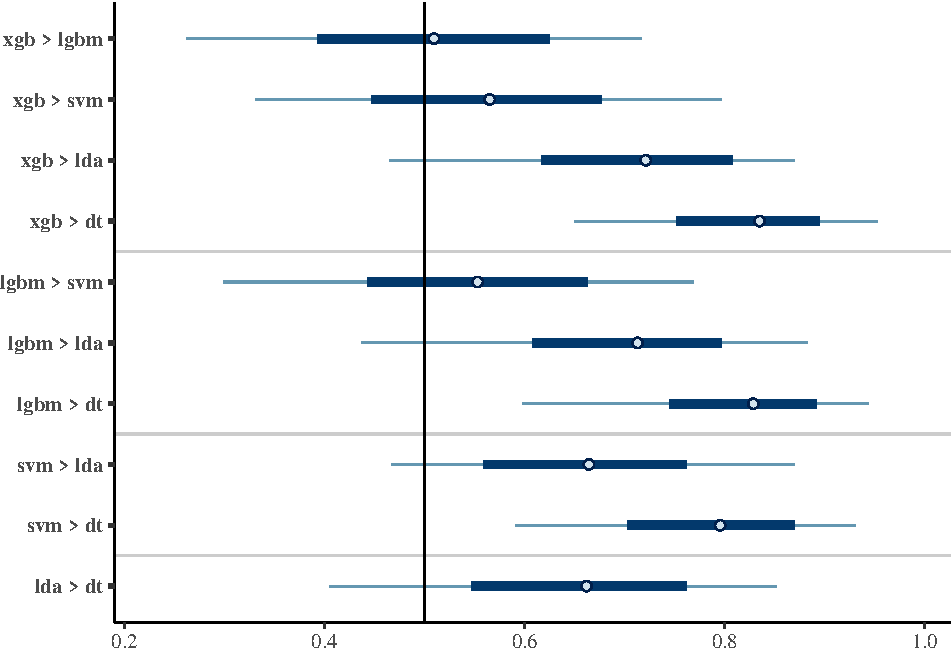
\includegraphics[width=0.7\linewidth]{figure_latex/xplot1-1} \caption{\label{fig:plot1}The graphical representation of the distribution of P (a better than b)}\label{fig:xplot1}
\end{figure}

Some of the data displayed in Figure \ref{fig:plot1} can be summarized in Table \ref{tab:main1}, containing the mean, the low and high limits of the 89\% HDI.

\begin{table}

\caption{\label{tab:xresume1}\label{tab:main1}The table representation of the distributions of probabilities}
\centering
\begin{tabular}[t]{lrrr}
\toprule
\textbf{pair} & \textbf{mean} & \textbf{low} & \textbf{high}\\
\midrule
\cellcolor{gray!6}{xgb > lgbm} & \cellcolor{gray!6}{0.51} & \cellcolor{gray!6}{0.40} & \cellcolor{gray!6}{0.63}\\
xgb > svm & 0.56 & 0.45 & 0.68\\
\cellcolor{gray!6}{xgb > lda} & \cellcolor{gray!6}{0.72} & \cellcolor{gray!6}{0.62} & \cellcolor{gray!6}{0.81}\\
xgb > dt & 0.83 & 0.75 & 0.90\\
\cellcolor{gray!6}{lgbm > svm} & \cellcolor{gray!6}{0.55} & \cellcolor{gray!6}{0.44} & \cellcolor{gray!6}{0.66}\\
\addlinespace
lgbm > lda & 0.71 & 0.62 & 0.81\\
\cellcolor{gray!6}{lgbm > dt} & \cellcolor{gray!6}{0.82} & \cellcolor{gray!6}{0.75} & \cellcolor{gray!6}{0.90}\\
svm > lda & 0.66 & 0.57 & 0.77\\
\cellcolor{gray!6}{svm > dt} & \cellcolor{gray!6}{0.79} & \cellcolor{gray!6}{0.72} & \cellcolor{gray!6}{0.88}\\
lda > dt & 0.66 & 0.56 & 0.77\\
\bottomrule
\end{tabular}
\end{table}

\hypertarget{convergence-diagnostics-and-execution-times}{%
\subsection{\texorpdfstring{Convergence Diagnostics and execution times \label{sec:conv1}}{Convergence Diagnostics and execution times }}\label{convergence-diagnostics-and-execution-times}}

As discussed, every run of an MCMC algorithm would possibly require
verifying that the algorithm did converge to the target distribution.
In this research, we use Stan \citep{stan229} as the language to describe
the BBT model (\ref{eq:mod1}) and to run the MCMC. Stan collects many
convergence diagnostics data and interprets them into claims on
whether there was an acceptable convergence or not. The result of
running the simplified Stan check is displayed below.

\begin{verbatim}
## Checking sampler transitions treedepth.
## Treedepth satisfactory for all transitions.
## 
## Checking sampler transitions for divergences.
## No divergent transitions found.
## 
## Checking E-BFMI - sampler transitions HMC potential energy.
## E-BFMI satisfactory.
## 
## Effective sample size satisfactory.
## 
## Split R-hat values satisfactory all parameters.
## 
## Processing complete, no problems detected.
\end{verbatim}

The MCMC sampling of the model is unproblematic -- in all examples in
this paper, including the ones in the sections below, we used 1000
steps of warm-up and 1000 steps of sampling, on 4 chains. In a modern
laptop, for example, an Intel i5 at 1.4 GHz, each chain takes in the
worse case 0.5 seconds and the four them can be run truly in parallel,
one in each core.

\hypertarget{posterior-predictive-check-and-waic}{%
\subsection{\texorpdfstring{Posterior Predictive Check and WAIC \label{sec:ppc1}}{Posterior Predictive Check and WAIC }}\label{posterior-predictive-check-and-waic}}

Figure \ref{fig:ppc1} is a usual way of displaying the posterior
predictive check. The plot shows the \texttt{win1} variables from the
wintable -- one for each pair of algorithms. The histogram represent the data generated by the Bayesian
model and the vertical bar, the actual value for that variable. If
model is a good generator of the actual data, then the real data will
be well centered in the histogram of possible values for that
variable.

\begin{figure}
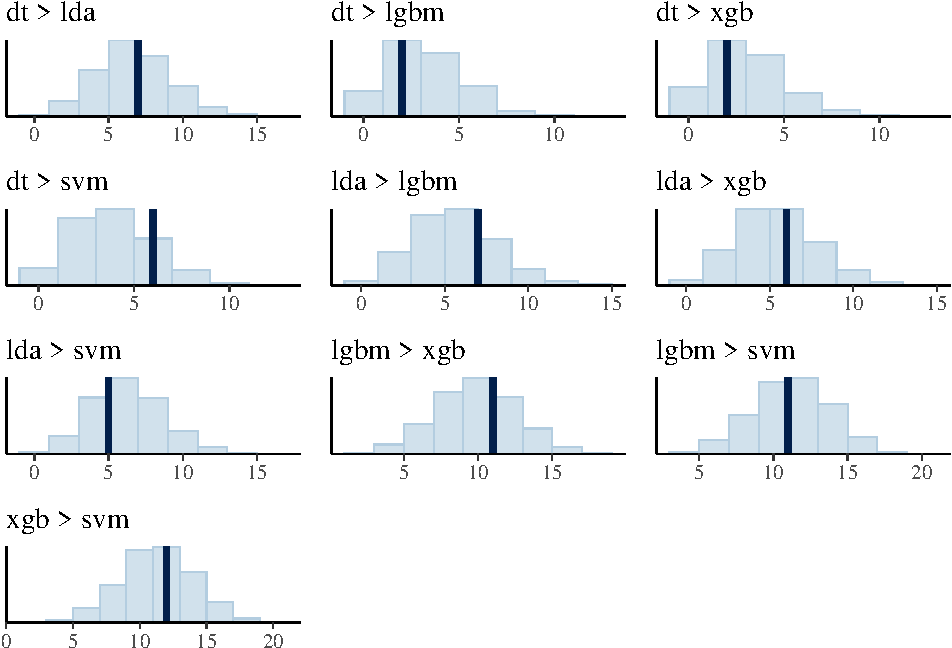
\includegraphics[width=0.7\linewidth]{figure_latex/xppc1-1} \caption{\label{fig:ppc1}Graphical representation of the PPC}\label{fig:xppc1}
\end{figure}

We also propose a non-graphical representation of the PPC: for each
variable we compute the 50\%, 90\%, 95\%, and 100\% HDI of the generated
values, and
compute the proportion of the true data what falls within each of its
own respective HDI. The proportion of data values that fall within
its respective 90\% HDI should be 0.9 or more. Table \ref{tab:ppc1}
displays this alternative representation of the PPC.

\begin{table}

\caption{\label{tab:xppc2}\label{tab:ppc1}The table representation of the PPC}
\centering
\begin{tabular}[t]{rr}
\toprule
\textbf{hdi} & \textbf{proportion}\\
\midrule
\cellcolor{gray!6}{0.50} & \cellcolor{gray!6}{0.8}\\
0.90 & 1.0\\
\cellcolor{gray!6}{0.95} & \cellcolor{gray!6}{1.0}\\
1.00 & 1.0\\
\bottomrule
\end{tabular}
\end{table}

\hypertarget{rope-1}{%
\subsection{\texorpdfstring{ROPE \label{sec:rope}}{ROPE }}\label{rope-1}}

As discussed above, the Bayesian perspective allows one to define a
difference between parameters that does not matter for practical
purposes, and to make statements regarding the probability that the
parameters do no differ in any practical sense.

The BBT model simplifies the adoption of the idea of practical
equivalence. The final measure of the BBT model is the probability
that a particular algorithm is better than some other. One can define
an universal ROPE for probability statements, regardless of underlying
metric being used to measure when one algorithm is ``better'' than
another. In this paper we propose that if the probability that one
algorithm is better than another is within the range of 0.45 to 0.55,
we can make the claim that the two algorithms are equivalent for
practical purposes.

Formally, if \(P(A \succ\,B) \in [0.45,0.55]\) we will make the claim
that algorithms \(A\) and \(B\) are equivalent for practical purposes.
This is not a claim based on the community's understanding of this
problem, or the author's experience in dealing with the comparison of
multiple algorithms. The ROPE limits are very easy to comprehend and
anyone can propose a different ROPE for different applications. The
author, somewhat arbitrarily, believes that an algorithm whose probability
of being better than another is below 55\% (and above 45\%) is really
not that better than the other one. Other researchers can have
different intuitions regarding this and are well justified to change
the ROPE for their application.

The ROPE can be included in both the distribution graph and the
summary table. In Figure \ref{fig:plot2}, the two gray vertical lines
represent the low and upper bound of the rope.

\begin{figure}
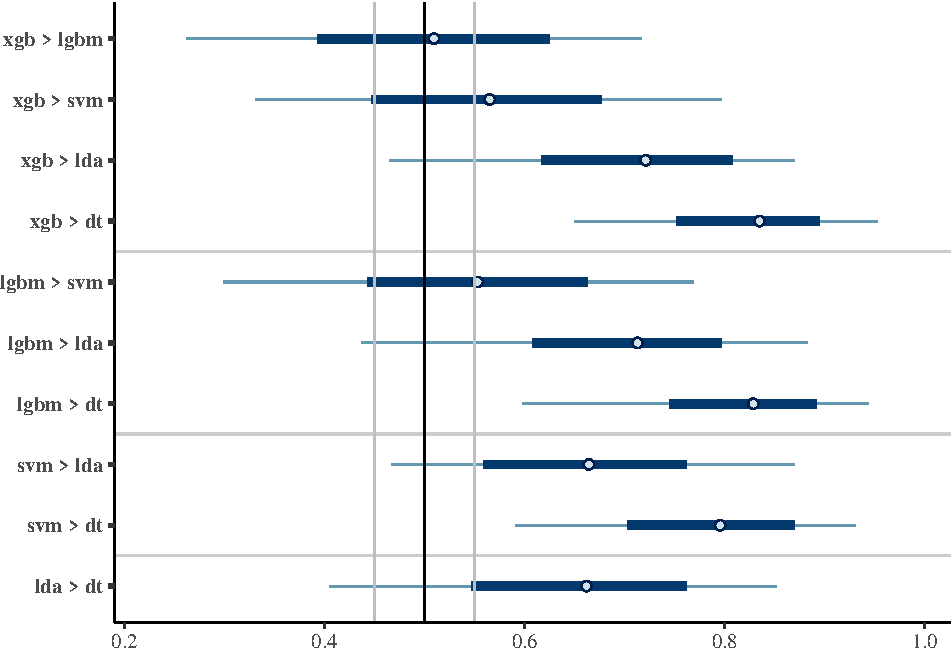
\includegraphics[width=0.7\linewidth]{figure_latex/xplot2-1} \caption{\label{fig:plot2}Graphical representation of the probability distributions with the rope information}\label{fig:xplot2}
\end{figure}

Table \ref{tab:main} is the summary of the probability distributions,
with two columns added. The {\em in.rope} column is the mass of
probability that \(A\) and \(B\) are equivalent for all practical
purposes, or more formally, the proportion of samples \(P_k(A \succ\,B)\) that fall within the ROPE interval \([0.45,0.55]\). The {\em above.50}
column is the mass of the probability distribution that \(A\) is better
than \(B\), or more formally, the proportion of samples \(P_k(A \succ\,B)\) that fall in the interval {[}0.50, 1.00{]}.

\begin{table}

\caption{\label{tab:xtaball2}\label{tab:main}Table with the summary of the probabilities distributions}
\centering
\begin{tabular}[t]{lrrrr}
\toprule
\textbf{pair} & \textbf{mean} & \textbf{delta} & \textbf{above.50} & \textbf{in.rope}\\
\midrule
\cellcolor{gray!6}{xgb > lgbm} & \cellcolor{gray!6}{0.51} & \cellcolor{gray!6}{0.23} & \cellcolor{gray!6}{0.56} & \cellcolor{gray!6}{0.51}\\
xgb > svm & 0.56 & 0.23 & 0.81 & 0.36\\
\cellcolor{gray!6}{xgb > lda} & \cellcolor{gray!6}{0.72} & \cellcolor{gray!6}{0.19} & \cellcolor{gray!6}{1.00} & \cellcolor{gray!6}{0.00}\\
xgb > dt & 0.83 & 0.14 & 1.00 & 0.00\\
\cellcolor{gray!6}{lgbm > svm} & \cellcolor{gray!6}{0.55} & \cellcolor{gray!6}{0.22} & \cellcolor{gray!6}{0.78} & \cellcolor{gray!6}{0.41}\\
\addlinespace
lgbm > lda & 0.71 & 0.19 & 1.00 & 0.01\\
\cellcolor{gray!6}{lgbm > dt} & \cellcolor{gray!6}{0.82} & \cellcolor{gray!6}{0.14} & \cellcolor{gray!6}{1.00} & \cellcolor{gray!6}{0.00}\\
svm > lda & 0.66 & 0.20 & 0.99 & 0.04\\
\cellcolor{gray!6}{svm > dt} & \cellcolor{gray!6}{0.79} & \cellcolor{gray!6}{0.16} & \cellcolor{gray!6}{1.00} & \cellcolor{gray!6}{0.00}\\
lda > dt & 0.66 & 0.21 & 0.99 & 0.06\\
\bottomrule
\end{tabular}
\end{table}

\hypertarget{strong-and-weak-interpretations-of-the-probability-estimates}{%
\subsubsection{\texorpdfstring{Strong and weak interpretations of the probability estimates \label{strong-weak}}{Strong and weak interpretations of the probability estimates }}\label{strong-and-weak-interpretations-of-the-probability-estimates}}

We believe that the four important columns to report are {\em mean},
{\em delta} (the difference between the {\em high} and {\em low} values of the HDI)
{\em in.rope} and {\em above.50}. In particular, the {\em mean} and the {\em above.50}
measures will be central to what we will call the \textbf{strong} and the
\textbf{weak interpretations} of the probability estimates. As discussed, the
BBT model generates a set of numbers \(P_k(A \succ\,B)\) which we have
been calling probabilities that \(A\) is better than \(B\). And in fact,
these numbers are used in the BBT model as the parameters of the
binomial distribution that are interpreted as probabilities of the
event happening. Under the strong interpretation, we do understand
these numbers as probabilities that \(A\) is better than \(B\) in a
frequentist approach - in the long run, for a large number of data
sets, the proportion of times \(A\) wins from \(B\) should approach that
number. In the strong interpretation, the {\em mean} column is the best estimation
of how much better algorithm A is from B. The {\em delta} column (or both
{\em low} and {\em high}) are the estimates on how uncertain one is about that
probability.

The weak interpretation sees each \(P_k(A \succ\,B)\) as a number that
measures how much A is better than B. It happens to be a number that
ranges from 0.0 to 1.0, and if the number is lower than 0.5, it
indicates that B is better than A. Under the weak interpretation, each
\(P_k(A \succ\,B)\) is an evidence that A is better than B, not a
promise of future proportions of wins in the long run. In this case,
the {\em above.50} is the measure on how confident one should be that A is
better than B. If 90\% of the evidence (each \(P_k(A \succ\,B)\)) are
above 0.5, one can be 90\% confident that A is better than B.

The {\em in.rope} measure falls oddly between the two
interpretations. Following the weak interpretation, we are counting
the proportion of evidence that falls within an interval (from 0.45 to
0.55). But to justify the range of the ROPE, we used a strong
interpretation's point of view: the fact that, in the long run, one
algorithm will win from the other at most 55\% of the time is not
relevant for practical purposes.

There are two reasons to put forth these two interpretations, and not
just to follow the more direct strong interpretation. In section
\ref{compare-tests} we will see that in order to compare the BBT model
with previous ones, we should use the weak interpretation; and in
section \ref{predictive} we will show that the BBT model
may not be very well calibrated for predictions on future results for the
algorithms under the strong interpretation, but it is better calibrated under the weak interpretation.

\hypertarget{comparisons-against-a-control}{%
\subsection{\texorpdfstring{Comparisons against a control \label{sec:control}}{Comparisons against a control }}\label{comparisons-against-a-control}}

In Bayesian tests, there is no need to distinguish between all
pairwise comparisons and comparisons against a control. There is no
penalty regarding the quality of assessments when performing only \(n\)
instead of \(n(n-1)/2\) pairwise comparisons. If one is only interested
in displaying the comparisons of the control algorithm against its
competitors, one need only to limit the rows of the summary table that
are shown.

Using the ll-results, let us assume that the \emph{xrf} algorithm is the control. One can run the full BBT model for all algorithms and display only the rows that include \emph{xrf}. Table \ref{tab:control} show these results

\begin{table}

\caption{\label{tab:control1}\label{tab:control}Table with the summary for the xrf control algorithm on the ll-results.}
\centering
\begin{tabular}[t]{lrrrr}
\toprule
\textbf{pair} & \textbf{mean} & \textbf{delta} & \textbf{above.50} & \textbf{in.rope}\\
\midrule
\cellcolor{gray!6}{rf > xrf} & \cellcolor{gray!6}{0.60} & \cellcolor{gray!6}{0.05} & \cellcolor{gray!6}{1.0} & \cellcolor{gray!6}{0.00}\\
lgbm > xrf & 0.59 & 0.05 & 1.0 & 0.01\\
\cellcolor{gray!6}{xgb > xrf} & \cellcolor{gray!6}{0.58} & \cellcolor{gray!6}{0.05} & \cellcolor{gray!6}{1.0} & \cellcolor{gray!6}{0.03}\\
gbm > xrf & 0.56 & 0.05 & 1.0 & 0.24\\
\cellcolor{gray!6}{mlp > xrf} & \cellcolor{gray!6}{0.54} & \cellcolor{gray!6}{0.05} & \cellcolor{gray!6}{1.0} & \cellcolor{gray!6}{0.65}\\
\addlinespace
xrf > svm & 0.51 & 0.05 & 0.8 & 0.99\\
\cellcolor{gray!6}{xrf > lr} & \cellcolor{gray!6}{0.58} & \cellcolor{gray!6}{0.05} & \cellcolor{gray!6}{1.0} & \cellcolor{gray!6}{0.04}\\
xrf > lda & 0.62 & 0.05 & 1.0 & 0.00\\
\cellcolor{gray!6}{xrf > svml} & \cellcolor{gray!6}{0.62} & \cellcolor{gray!6}{0.05} & \cellcolor{gray!6}{1.0} & \cellcolor{gray!6}{0.00}\\
xrf > ridge & 0.68 & 0.05 & 1.0 & 0.00\\
\addlinespace
\cellcolor{gray!6}{xrf > knn} & \cellcolor{gray!6}{0.69} & \cellcolor{gray!6}{0.05} & \cellcolor{gray!6}{1.0} & \cellcolor{gray!6}{0.00}\\
xrf > dt & 0.72 & 0.04 & 1.0 & 0.00\\
\cellcolor{gray!6}{xrf > qda} & \cellcolor{gray!6}{0.77} & \cellcolor{gray!6}{0.04} & \cellcolor{gray!6}{1.0} & \cellcolor{gray!6}{0.00}\\
xrf > nb & 0.82 & 0.03 & 1.0 & 0.00\\
\cellcolor{gray!6}{xrf > passive} & \cellcolor{gray!6}{0.85} & \cellcolor{gray!6}{0.03} & \cellcolor{gray!6}{1.0} & \cellcolor{gray!6}{0.00}\\
\bottomrule
\end{tabular}
\end{table}

\hypertarget{what-counts-as-a-win-folds-and-local-rope}{%
\section{\texorpdfstring{What counts as a win? Folds and local rope \label{sec:lrope}}{What counts as a win? Folds and local rope }}\label{what-counts-as-a-win-folds-and-local-rope}}

Usually, the final performance measure for a particular algorithm for
a particular data set is the average of the measures on some form of
repeated cross validation, where the algorithm trains on different
subsets of the data set and its performance is measured on the
corresponding test subsets. Standard forms of repeated
cross-validations are: k-fold, repeated k-folds, repeated train/test
split, and bootstrapped samples of the data set. In each case, there
are \(k\) pairs of subsets \(TR_i\) (train) and \(TE_i\) (test) such that
\(TR_i \cup TE_i = DS\) and \(TR_i \cap TE_i = \emptyset\) (\(DS\) is the
whole data set). We will call each of the \(TE_i\) as a \textbf{fold}
although we do not assume that a k-fold cross validation is being
used -- almost all cross-validation procedures can be used.

Regarding the data in this research, we computed the mean of a 4-fold
cross-validation of each algorithm for each data set. Furthermore,
for each data set the folds were fixed and the same for all
algorithms, that is, for the first fold, all algorithms were trained
in the subset \(TR_1\) and tested in the subset \(TE_1\), and so on.

Let us consider a particular pair of measures from table \ref{tab:sstab1} for the
data set ``cmc'' repeated as Table \ref{tab:small1}. The entries for
the \emph{lgbm} and the \emph{xgb} algorithms are 0.525 and 0.524 respectively.
This small difference counts as a win for \emph{lgbm}, as much as the much
more impressive difference to the 0.455 accuracy for the \emph{dt}
algorithm also counts as a win.

\begin{table}

\caption{\label{tab:xsmall1}\label{tab:small1}Detail of the base results for the cmc data set}
\centering
\begin{tabular}[t]{lrrrrr}
\toprule
\textbf{db} & \textbf{dt} & \textbf{lda} & \textbf{lgbm} & \textbf{xgb} & \textbf{svm}\\
\midrule
cmc & 0.455 & 0.513 & 0.525 & 0.524 & 0.544\\
\bottomrule
\end{tabular}
\end{table}

If we consider the folds themselves for the ``cmc'' data set, displayed
in table \ref{tab:small2}, we see that this small difference is
even less convincing as a win for the \emph{lgbm} algorithm. For these
runs, we used the same fold 1, fold 2, and so on for all the
algorithms, and thus it is reasonable to compare the performance of
the algorithms on each fold separately. In this case, \emph{lgbm} wins on
two of the folds, but looses on the other two, of the 4 fold
computation of the algorithm's accuracy. Therefore, if we use the
folds as sources of evidence instead of working on the mean of the
folds' results, \emph{lgbm} would receive two wins and \emph{xgb} also have to
wins, as opposed to a single win for \emph{lgbm} when using the means.

From another point of view, if we consider the standard deviations of
the measures on the folds for each algorithm, also displayed on Table
\ref{tab:small2}, the differences in the mean of both algorithms
(0.001) is also much smaller than the standard deviations (0.02 and
0.03). In some intuitive sense, the difference in averages that
yielded the win for \emph{lgbm} is much smaller than some ``noise level'' of
the evaluation procedure itself, considering the variability of the
measures in the folds within each classifier itself.

This opens up two lines of reasoning: the one that considers each fold
(provided they are the same for all algorithms) as sources of evidence
to count the wins and losses of the algorithms, and one that deals
with the difference between the means for all folds, but take into
consideration both the difference and some ``noise level'' derived from
the variability within each classifier. But in both cases we are
aiming reducing the strength of evidence that \emph{lgbm} has a victory in
relation to \emph{xgb}, and that should be considered a tie.

This research will follow the ``noise level'' line. We argue that a
difference of 0.001 in the means given that for each classifier the
variability of the measures in the folds is at least 10 times as high,
should not count as a win but as a ties between the two algorithms.
We will call this approach the \textbf{local ROPE}, some threshold below
which one should consider the difference between two classifiers as
unimportant. But as we will see, the local ROPE is not a fixed number but
depend on the results of the two algorithms on the different folds.

Regarding the first line, using the folds themselves as source of
evidence for wins and losses, we believe that issues such as the fact
that the fold results are not independent of each other would make the
analysis too complex (the same conclusion reached by \citet{benavoli2017time}
for their analysis), and will leave that approach for future research.

\begin{table}

\caption{\label{tab:xsmall2}\label{tab:small2}Detail of the base results for the cmc data set}
\centering
\begin{tabular}[t]{llrrr}
\toprule
\textbf{db} & \textbf{fold} & \textbf{lgbm} & \textbf{xgb} & \textbf{diff}\\
\midrule
cmc & 1 & 0.547 & 0.531 & 0.016\\
cmc & 2 & 0.522 & 0.538 & -0.016\\
cmc & 3 & 0.503 & 0.481 & 0.022\\
cmc & 4 & 0.527 & 0.546 & -0.019\\
sd &  & 0.018 & 0.029 & 0.001\\
\bottomrule
\end{tabular}
\end{table}

\hypertarget{local-rope}{%
\subsection{\texorpdfstring{Local ROPE \label{localrope}}{Local ROPE }}\label{local-rope}}

In almost all statistical tests one has two sets of measures, and one
wants to make a claim regarding whether there is enough evidence that
the difference of the means (or other summary measure) of the two sets is ``real'' or not. This
is exactly the problem in hand: should one consider the difference of
the means of the folds as ``real'' -- and thus that one algorithm is
better than the other -- or not?

Cohen's D is a measure of effect size between two sets of data. For
the case where the two sets have the same number of data, as it is our
case, the Cohen d is computed as the difference between the means,
divided by an ``average'' standard deviation of the two sets, where the
``average'' standard deviation is actually the square root of the average
variance of the two sets. This is displayed in Equation \ref{eq:d}.
Cohen d is the measure of the separation between the two means, as a
proportion of the standard deviation and can be seen as a signal
to noise ratio measure: the difference in means is the signal, and the
``average'' standard deviation is the noise.

\begin{equation} \label{eq:d}
d = \frac{\mu_1 - \mu_2}{\sqrt{\frac{\sigma_1^2 + \sigma_2^2}{2}}} 
\end{equation}

We can compute the Cohen D of two set of fold measures, and consider
that there is no important difference, and thus, a ties between the two
algorithms, if the D is below a threshold \(d_{\min}\) which we will
call the \textbf{local ROPE threshold}. Therefore, if:

\begin{equation} \label{eq:dmin}
\mu_1 - \mu_2 \le d_{\min} \sqrt{\frac{\sigma_1^2 + \sigma_2^2}{2}} 
\end{equation}

we should consider that there was a tie between algorithms 1 and 2 for that data set.

We will argue that the threshold can be safely set to the value of 0.4
using the theory of power analysis for t-tests. We refer the reader to the concepts of type 1 and type 2 errors, their probabilities \(\alpha\) and \(\beta\) (section \ref{sec:tut1}).
The power analysis of t-tests relates \(\alpha\), \(\beta\), the effect
size of the measure, and the number of samples in each set.
Unfortunately, the relation between these variables is almost never
displayed as an equation, but as tables \citep[ch.~2]{cohen1988statistical}
or embedded into programs, such as G*power \citep{faul2007g} or
the \texttt{pwr} R package \citep{pwrR}. We will show the results of running the
\texttt{pwr} package.

For our present goals, there is no conceptual difference
between false positive and false negative errors. We want to find out
whether the two sets of fold measures indicate that the difference
between the means is ``real'' or ``not real'', and erring to one side is
not worse that to the other. Thus, let us assume a 70\% probability of
detecting both the presence of a real difference and a absence of a
real non-difference, that is, \(\alpha = 0.3\) and \(\beta = 0.3\). For
this case, and assuming a Cohen D of 0.4, the necessary number of data
in each set is given by running the \texttt{pwr} function:

\begin{quote}
\begin{verbatim}
 pwr.t.test(n = NULL, d = 0.4, sig.level = 0.3, power = 0.7)

 Two-sample t test power calculation 
           n = 30.18637
           d = 0.4
   sig.level = 0.3
       power = 0.7
 alternative = two.sided
 NOTE: n is number in *each* group
\end{verbatim}
\end{quote}

In this case one would need at least 30 measure in each set to be able
to find a true difference or a true non-difference with 70\%
probability. But the traditional cross validations in machine
learning are from 3 to 10 folds. That is, using the usual cross
validation in machine learning, a minimum effect size of 0.4 is very
safe - one would not be able to detect differences whose effect sizes
are 0.4 or below, if one requires a 70\% of sensitivity and
specificity. If one is using 10 repetitions of 10-folds as cross
validation, one can use \(d_{\min} = 0.2\).

The discussion above assumes that the two samples of fold measures are
not paired, that is, that possible different
folds were used in the evaluation of the different algorithms. But if
the researchers have control over it, they can use the same folds for
all algorithms. For the paired case, the definition of
the Cohen's D is somewhat different than the one presented in
\ref{eq:d}. Instead of dealing with the mean and standard deviations
of the two sets, one should compute the mean and standard deviation of
the differences between the corresponding paired data in the two sets.

\begin{equation} \label{eq:dz}
d_z = \frac{\mu_{X_1 - X_2}}{\sigma_{X_1 - X_2}} = \frac{\mu_1 - \mu_2}{\sigma_{X_1 - X_2}} 
\end{equation}

The power analysis for paired samples is also somewhat different, and
with the same numbers as before (\(\alpha = 0.3\) and \(\beta = 0.3\)),
and using Equation \ref{eq:dz} for the effect size calculation, the
resulting lower bound for the number of samples is 15, lower than the
case for unrelated samples, but still well above the usual number of
folds used in machine learning evaluations.

\begin{quote}
\begin{verbatim}
  pwr.t.test(n = NULL, d = 0.4, sig.level = 0.3, power = 0.7, type="paired")

  Paired t test power calculation 
           n = 15.53464
           d = 0.4
   sig.level = 0.3
       power = 0.7
 alternative = two.sided
 NOTE: n is number of *pairs*
\end{verbatim}
\end{quote}

The same decision process as described in \ref{eq:dmin} can be
followed, using the same \(d_{min}\) threshold of 0.4, but using the
paired definition for the effect size.

\begin{equation} \label{eq:dmin2}
\mu_1 - \mu_2 \le d_{\min} \sigma_{X_1 - X_2}
\end{equation}

\hypertarget{how-to-deal-with-ties}{%
\subsection{\texorpdfstring{How to deal with ties? \label{test-ties}}{How to deal with ties? }}\label{how-to-deal-with-ties}}

The local ROPE concept introduces many ties to the wintable, as it is designed to do.
The standard ways of dealing with ties in the Bradley-Terry model are:

\begin{itemize}
\tightlist
\item
  add: add the ties as victories to both players involved.
\item
  spread: add the ties as half a victory to each player involved
\item
  forget: do not add ties to as victories to any of the players.
\end{itemize}

Another alternative is to change the Bradley-Terry model into a model
that includes ties, for example the one proposed by
\citet{davidson1970extending}. The Davidson model is displayed in Equation
\ref{eq:david}. It includes a new parameter \(\nu\) similar to the
\(\beta_i\). \(\nu\) controls how likely are ties ``in that sport'', despite the differences
between the players. If \(\nu \rightarrow -\infty\), \(P( i \mbox{~ties~} j)\) will be 0, that is, there are no ties; if \(\nu \rightarrow \infty\), \(P( i \mbox{ties} j)\) will be 1, regardless of
the players' different \(\beta\). Finally, for \(\nu = 0\), if \(\beta_i = \beta_j\) then the probability of a tie is \(1/3\).

\begin{align}
 P(i \succ\,j | \mbox{~no tie~}) &= \frac{\exp \beta_i}{\exp \beta_i +\exp \beta_j + \exp(\nu + (\beta_i + \beta_j)/2) }  \label{eq:david}\\
P( i \mbox{~ties~} j) &= \frac{\exp (\nu + (\beta_i + \beta_j)/2) }{\exp \beta_i +\exp \beta_j + \exp (\nu + (\beta_i + \beta_j)/2 ) } \nonumber
\end{align}

We will compare the different policies, using a repeated experiment as
described above, and comparing how well the different solutions model
the data. We will use the posterior predictive check and the WAIC to measure
how well each policy fits the real data. Regarding the WAIC, the
number itself is hard to interpret, but when comparing two models, the
lower the value of the WAIC, the better (as it is with other
information measures such as AIC and BIC).

Tables \ref{tab:tiesppc1} and \ref{tab:tiesppc1b} display the WAIC,
and the PPC summary results for the repeated experiments for comparing
different ways of dealing with ties. The results are the average of
the repeated experiments on ss, mm, sl use cases, and the ll-results,
also averaging whether the local ROPE was used or not, and whether the
paired local ROPE was used. The results clearly show that the Davidson
model is much worse than the others regarding both WAIC and
PPC. Add, forget and spread policies are all equivalent, and somewhat
arbitrarily, we decided on using the spread policy in this paper.

The low quality of the Davidson model is somewhat surprising, given
that the model explicitly deals with ties, and the other policies
seems \emph{ad hoc} solutions. Table \ref{tab:tiesppc2} show the
results of the PPC summary for the ll-results. One can see that
neither the wins nor the ties are well calibrated with their
corresponding HDI.

\begin{table}

\caption{\label{tab:tiesxz1}\label{tab:tiesppc1}The PPC of ss and mm use cases for the different policies.}
\centering
\begin{tabular}[t]{lrrrrrrrrrr}
\toprule
\multicolumn{1}{c}{ } & \multicolumn{5}{c}{ss} & \multicolumn{5}{c}{mm} \\
\cmidrule(l{3pt}r{3pt}){2-6} \cmidrule(l{3pt}r{3pt}){7-11}
\textbf{\textbf{policy}} & \textbf{\textbf{waic}} & \textbf{\textbf{h50}} & \textbf{\textbf{h90}} & \textbf{\textbf{h95}} & \textbf{\textbf{h100}} & \textbf{\textbf{waic}} & \textbf{\textbf{h50}} & \textbf{\textbf{h90}} & \textbf{\textbf{h95}} & \textbf{\textbf{h100}}\\
\midrule
add & 42.41 & 0.87 & 1.00 & 1.00 & 1 & 225.51 & 0.73 & 1.00 & 1.00 & 1.00\\
davidson & 118.59 & 0.40 & 0.78 & 0.86 & 1 & 873.01 & 0.29 & 0.58 & 0.66 & 0.88\\
forget & 40.27 & 0.78 & 0.99 & 1.00 & 1 & 227.61 & 0.61 & 0.96 & 0.99 & 1.00\\
spread & 41.41 & 0.82 & 1.00 & 1.00 & 1 & 223.76 & 0.68 & 0.99 & 1.00 & 1.00\\
\bottomrule
\end{tabular}
\end{table}

\begin{table}

\caption{\label{tab:tiesxz2}\label{tab:tiesppc1b}The PPC of sl and ll use cases the different policies.}
\centering
\begin{tabular}[t]{lrrrrrrrrrr}
\toprule
\multicolumn{1}{c}{ } & \multicolumn{5}{c}{sl} & \multicolumn{5}{c}{ll} \\
\cmidrule(l{3pt}r{3pt}){2-6} \cmidrule(l{3pt}r{3pt}){7-11}
\textbf{\textbf{policy}} & \textbf{\textbf{waic}} & \textbf{\textbf{h50}} & \textbf{\textbf{h90}} & \textbf{\textbf{h95}} & \textbf{\textbf{h100}} & \textbf{\textbf{waic}} & \textbf{\textbf{h50}} & \textbf{\textbf{h90}} & \textbf{\textbf{h95}} & \textbf{\textbf{h100}}\\
\midrule
add & 61.62 & 0.81 & 0.97 & 0.99 & 1.00 & 760.49 & 0.57 & 0.95 & 0.97 & 1.00\\
davidson & 325.65 & 0.21 & 0.51 & 0.56 & 0.78 & 4730.36 & 0.17 & 0.38 & 0.43 & 0.70\\
forget & 65.46 & 0.67 & 0.95 & 0.97 & 0.99 & 823.52 & 0.39 & 0.85 & 0.91 & 0.99\\
spread & 62.25 & 0.75 & 0.97 & 0.99 & 1.00 & 773.98 & 0.47 & 0.92 & 0.95 & 1.00\\
\bottomrule
\end{tabular}
\end{table}

\begin{table}

\caption{\label{tab:ties2}\label{tab:tiesppc2} The Davidson model on the ll-results.}
\centering
\begin{tabular}[t]{rrr}
\toprule
\textbf{hdi} & \textbf{proportion} & \textbf{ties}\\
\midrule
0.50 & 0.23 & 0.26\\
0.90 & 0.46 & 0.46\\
0.95 & 0.52 & 0.49\\
1.00 & 0.91 & 0.82\\
\bottomrule
\end{tabular}
\end{table}

\hypertarget{comparison-with-standard-approaches}{%
\section{\texorpdfstring{Comparison with standard approaches \label{compare-tests}}{Comparison with standard approaches }}\label{comparison-with-standard-approaches}}

Let us compare the results of using the BBT procedure with that of using some of the standard comparisons procedures. Section \ref{sec:comp-demsar} compare the BBT with Demsar's procedure on a different set of use-cases; section \ref{sec:comp-wil} compares with the pairwise Wilcoxon procedure, and section \ref{sec:comp-bsr} compares with the Bayesian signed rank procedure.

\hypertarget{demsars}{%
\subsection{\texorpdfstring{Demsar's \label{sec:comp-demsar}}{Demsar's }}\label{demsars}}

The Demsar's procedure starts with the evaluation of the Friedman test, which results in a p-value \(\le 0.05\) for the base results.
The next step is the Nemenyi test, which results in the Critical Difference plot displayed in Figure \ref{fig:demsar1}.
The results of significant and non significant differences can be displayed in a tabular for as in
Table \ref{tab:demsar22}.

\begin{figure}
\begin{floatrow}
\ffigbox{%
  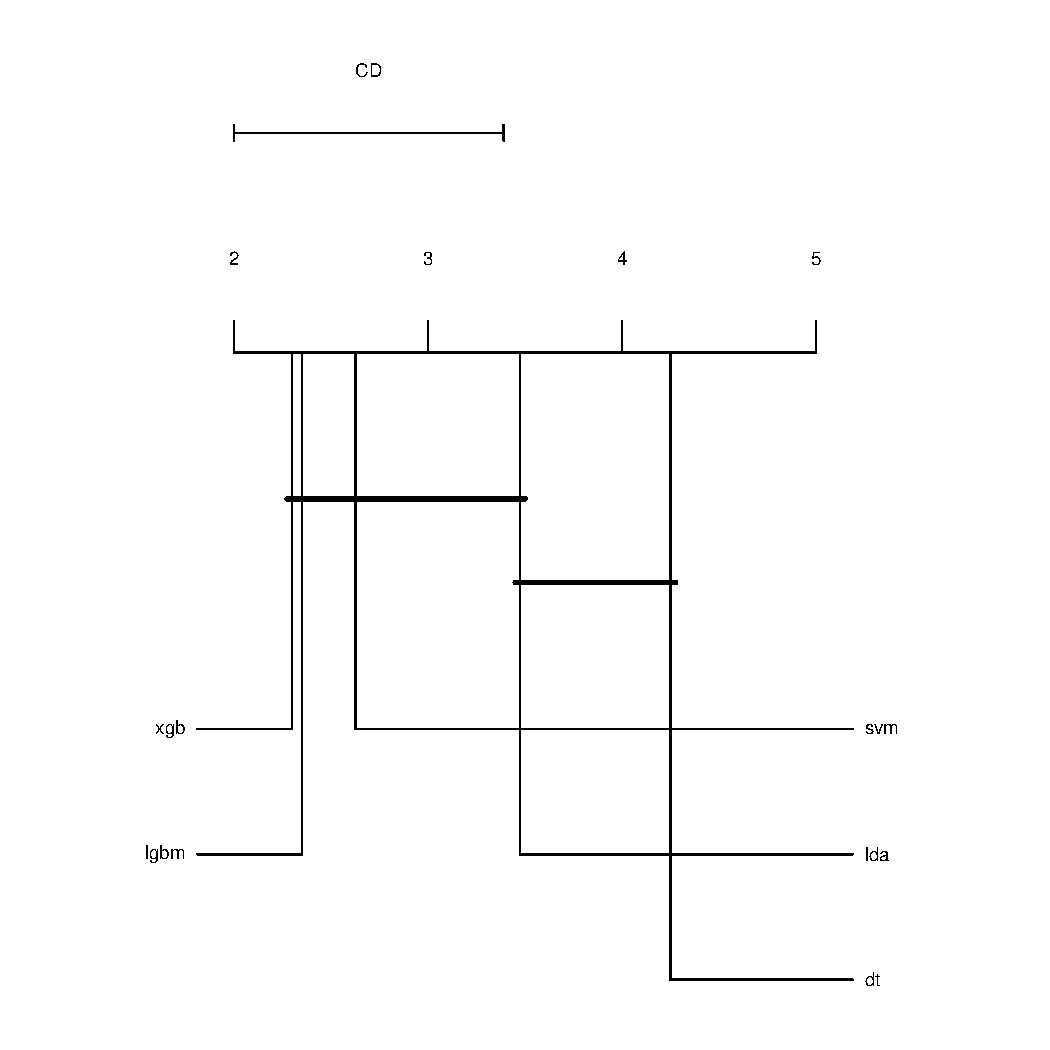
\includegraphics[scale=0.5]{figure_latex/cdplot.pdf}%
}{%
  \caption{The CD plot of the base results}\label{fig:demsar1}.%
}
\capbtabbox{%
% latex table generated in R 4.3.0 by xtable 1.8-4 package
% Thu Jul 13 15:59:18 2023
\begin{tabular}{lr}
  \toprule
{\bfseries algorithm} & {\bfseries mean rank} \\ 
  \midrule
xgb & 2.30 \\ 
  lgbm & 2.35 \\ 
  svm & 2.62 \\ 
  lda & 3.48 \\ 
  dt & 4.25 \\ 
   \bottomrule
\end{tabular}

}{%
  \caption{The table representation of the CD plot}\label{tab:demsar22}%
}
\end{floatrow}
\end{figure}

We refer the reader to Table \ref{tab:main} for the BBT results regarding the base results. Here, we are faced with the strong vs weak interpretations of the probability estimates. Under the \emph{strong} interpretation, it would be reasonable to make an equivalence between a frequentist test making a claim of statistical significant difference between algorithm A and B (with 95\% confidence) and that the mean estimate that \(P(A \succ\,B) \ge 0.95\). These two concepts are not the same, but it is reasonable to make the equivalence to compare them. In this case, none of the claims of superiority made by the BBT model reaches the level of 95\%. The highest mean is 0.84 (\emph{xgb} against \emph{dt}).

But under the weak interpretation, using {\em above.50} \(\ge 0.95\) as the equivalence of statistical significance, the BBT procedure finds 5 differences that one would call significant, as opposed to three found by the Demsar's procedure.
In the base results, the differences between \emph{lgbm} and \emph{lda}, and \emph{xgb} and \emph{lda} are detected as ``significant'' by BBT, but they were not detected as such by the Demsar's procedure.

We ran the repeated experiments to verify how frequent are three results when comparing the BBT model with the traditional frequentist approach proposed by Demsar: how many times does BBT find a significant difference (in the sense that the {\em above.50} result is larger than 0.95) where Demsar does not find it significant, how many times the reverse happens, and how many times the aggregated ranking computed by one method did agree with the one computed by the other method.

The results are:

\begin{itemize}
\item
  \emph{ss:} For the 100 pairs of comparisons (10 from each ss), the BBT
  method classified 40 of them as significantly different, when
  Demsar did not determined them to be. No pairs were found
  significantly different by Demsar's procedure and not by BBT. Finally,
  only 3 of the 10 aggregated rankings were found to be the same.
\item
  \emph{mm:} For the 450 pairs, BBT found 187 that were not significant
  according to the Demsar procedure, none the other way, and 5 of
  the 10 aggregated rankings were the same.
\item
  \emph{sl:} For the 50 pairs, 11 were found as significant only by BBT
  and none the other way, and 5 aggregated rankings were in
  agreement.
\item
  \emph{ll results:} For 120 pairs of comparisons, BBT found 41 that were
  not significant by Demsar's, none the other way, and the
  aggregated ranking did not agree.
\end{itemize}

Thus there is strong evidence that the BBT procedure is stronger, in
the sense that it finds more significant differences than Demsar's
procedure, and that it supersedes Demsar's procedure, in the sense
that it does not miss any significant difference determined by
Demsar's. Furthermore, usually 50\% of the time, the two procedures do
not fully agree on the final aggregated ranking.

For all but the ll-results, there was no case in which {\em in.rope}
\(\ge 0.95\). For the ll results, there were 8 cases in which the
Demsar's procedure sees not significant difference but the BBT can
make a stronger claim that the two algorithms are equivalent. There is
an interesting case, which did not occur with our data, but
\citet{benavoli2017time} report, of two algorithms whose difference is
significant but are practically equivalent. The frequentist approach
has enough evidence to claim that the algorithms are different, but
the Bayesian approach claims that the difference does not matter! But
this is expected: with enough data all algorithms will be found
statistically different from each other, even those whose difference
is irrelevant.

\hypertarget{pairwise-wilcoxon}{%
\subsection{\texorpdfstring{Pairwise Wilcoxon \label{sec:comp-wil}}{Pairwise Wilcoxon }}\label{pairwise-wilcoxon}}

Table \ref{tab:wilcox22} reports the result of the pairwise Wilcoxon
tests, using the Horchberg p-value adjustment procedure. The column
{\em p-value} indicates the adjusted p-value of the comparison, and as
usual, the comparisons where p.value \(\le 0.05\) are considered
significant.

\begin{table}[ht]
\centering
\subfloat[Pairwise Wilcoxon: Order of the algorithms]{\scalebox{1.0}{% latex table generated in R 4.3.0 by xtable 1.8-4 package
% Thu Jul 13 15:59:19 2023
\begin{tabular}{lr}
  \toprule
{\bfseries algorithm} & {\bfseries median} \\ 
  \midrule
lgbm & 0.93 \\ 
  svm & 0.93 \\ 
  xgb & 0.93 \\ 
  dt & 0.87 \\ 
  lda & 0.85 \\ 
   \bottomrule
\end{tabular}
}}\quad
\subfloat[Pairwise Wilcoxon: Significance of differences displayed as a table.]{\label{tab:pairwil1}\scalebox{1.0}{% latex table generated in R 4.3.0 by xtable 1.8-4 package
% Thu Jul 13 15:59:19 2023
\begin{tabular}{lr}
  \toprule
{\bfseries name} & {\bfseries p.value} \\ 
  \midrule
lgbm $>$ svm & 0.98 \\ 
  lgbm $>$ xgb & 0.98 \\ 
  lgbm $>$ dt & 0.00 \\ 
  lgbm $>$ lda & 0.47 \\ 
  svm $>$ xgb & 0.98 \\ 
  svm $>$ dt & 0.11 \\ 
  svm $>$ lda & 0.46 \\ 
  xgb $>$ dt & 0.00 \\ 
  xgb $>$ lda & 0.46 \\ 
  dt $>$ lda & 0.98 \\ 
   \bottomrule
\end{tabular}
}}
\caption{Pairwise Wilcoxon tests - order of the algorithms and significance of differences displayed as a table."}
\label{tab:wilcox22}
\end{table}

Following the same procedure described above of considering
{\em above.50} \(\ge 0.95\) as ``equivalent'' to p.value \(\le 0.05\), we
see that the pairwise Wilcoxon tests only detect two significant
differences, for the five detected by the BBT model. Also the
aggregated rank is not the same for the pairwise Wilcoxon and BBT. The
second and third best algorithms, and the fourth and fifth (according
to BBT) are in reverse order for the pairwise Wilcoxon procedure,
although it does not find these to pairs of algorithms as
significantly different from each other.

We ran the replication experiments as above and
the results are:

\begin{itemize}
\item
  \emph{ss:} For the 100 pairs the BBT found 21 beyond the pairwise
  Wilcoxon, only one pair was detected by the pairwise Wilcoxon and
  missed by the BBT, and 2 of the 10 aggregated ranking were the
  same.
\item
  \emph{mm:} For the 450 pairs, BBT found 126 beyond the pairwise
  Wilcoxon, 6 missed, and no aggregated ranking was the same.
\item
  \emph{sl:} For the 50 pairs, BBT found 6 beyond the pairwise Wilcoxon,
  1 missed, and only one aggregated ranking was the same.
\item
  \emph{ll results:} For 120 pairs of comparisons, BBT found 21 beyond
  the pairwise Wilcoxon, 1 missed, and the methods did not agree on
  the aggregated ranking.
\end{itemize}

BBT seems to be stronger than the pairwise Wilcoxon but not all pairs
deemed significant by the pairwise Wilcoxon are found by BBT. The two
procedures fully agree on very few of the aggregated rankings. Also,
for the ll-results, there were 7 cases in which the pairwise Wilcoxon
procedure sees not significant difference but the BBT can make a
stronger claim that the two algorithms are equivalent.

\hypertarget{pairwise-bayesian-signed-rank}{%
\subsection{\texorpdfstring{Pairwise Bayesian signed rank \label{sec:comp-bsr}}{Pairwise Bayesian signed rank }}\label{pairwise-bayesian-signed-rank}}

Following the caveat that it is unclear whether one should use the
Bayesian signed rank (BSR) on multiple comparisons, Table
\ref{tab:pairbays1} displays the results of the
comparisons. \citet{benavoli2017time} suggest that one should report the
probabilities that the difference falls within the 0.1 ROPE
({\em in.rope}) and the probability that it falls above the ROPE
({\em above.rope}). We also report the probability that the
probability is above 0 ({\em above.0}), that is, that the difference
between the two mean parameter values is positive, that is, that one
algorithm is better than the other.

We believe that the only fair comparison is between the
{\em above.50} from BBT and the {\em above0} from BSR. Both measures
have the same semantics: {\em above0} counts the proportion of
evidence within BSR that one algorithm is better
than another and {\em above.50} under the weak interpretation also
counts the proportion of evidence that one algorithm is better than
another. Figure \ref{fig:bsr} plot the BSR {\em above0} measure against the
corresponding BBT {\em above.50} measure, where the dark line is the
\(y=x\) line. The figure also displays the Pearson correlation
coefficient of the two measures. As one can verify, there is a low
correlation between the results.

We do not know how to interpret the differences between the two
procedures, nor if the differences are important or not.

\begin{table}

\caption{\label{tab:xpairbays1}\label{tab:pairbays1}Results of the pairwise Bayesian Wilcoxon test}
\centering
\begin{tabular}[t]{lrrr}
\toprule
\textbf{name} & \textbf{above0} & \textbf{in.rope} & \textbf{above.rope}\\
\midrule
lgbm > svm & 0.72 & 0.62 & 0.33\\
lgbm > xgb & 0.50 & 1.00 & 0.00\\
lgbm > dt & 1.00 & 0.00 & 1.00\\
lgbm > lda & 0.95 & 0.01 & 0.96\\
svm > xgb & 0.21 & 0.60 & 0.06\\
\addlinespace
svm > dt & 1.00 & 0.00 & 1.00\\
svm > lda & 0.97 & 0.03 & 0.93\\
xgb > dt & 1.00 & 0.00 & 1.00\\
xgb > lda & 0.98 & 0.01 & 0.96\\
dt > lda & 0.20 & 0.00 & 0.24\\
\bottomrule
\end{tabular}
\end{table}

\begin{figure}
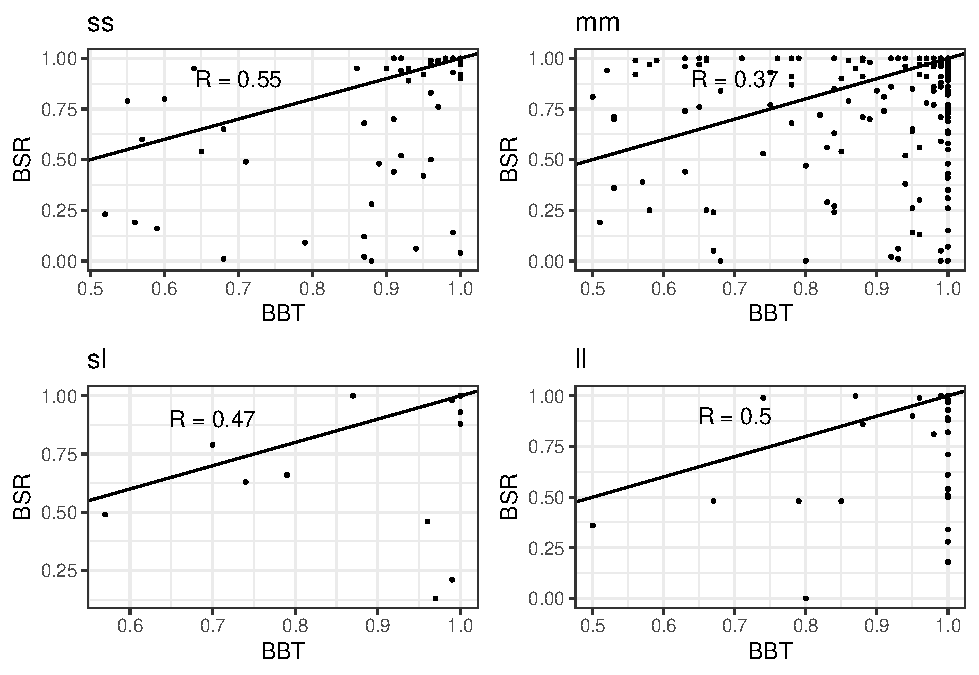
\includegraphics[width=0.9\linewidth]{figure_latex/bsr1-1} \caption{\label{fig:bsr}Comparison of the above0 from BSR and {\em above.50} (BBT) for the ss, mm , sl and ll use cases}\label{fig:bsr1}
\end{figure}

\hypertarget{bbt-as-a-prediction}{%
\section{\texorpdfstring{BBT as a prediction \label{predictive}}{BBT as a prediction }}\label{bbt-as-a-prediction}}

Frequentist methods are \emph{explanatory} in the sense that they explain
the data at hand, but they make no prediction about future data. The fact
that the difference between two sets of data is found not to be
significant is not a prediction (with 95\% probability, for example)
that future data for these sets will not be different from each
other. Instances of new data are almost always different from each other. Furthermore,
with more data, maybe the difference that was found not to be
significant becomes significant!

Frequentist tests do not make predictions, but Bayesian tests can. In
particular the BBT model's output as displayed in Table
\ref{tab:main}) can be seen as probabilities that one algorithm will better than
the others \emph{on future data}. There are two distinct predictions, as
discussed in section \ref{strong-weak}. In the strong interpretation,
the {\em mean} measure is a prediction of the proportion of wins for the
better algorithm against the worse for future data
sets. In the weak interpretation, the {\em above.50} is the prediction of
the proportion of wins for the better algorithm against the worse. In
this section we will test both predictions.

We ran the usual set of repeated experiments, but with the goal of
measuring how correct are these predictions on future data sets. For each sample of an
ss results (the ``training'' case), we also sampled 10 data sets not
used in the training ss, and measure in this ``test'' case, for each
pair of algorithms, the number of times one algorithm was better than
the other. For algorithms A1 and A2, let us call \emph{win1} the number of data sets for which
algorithm A1 performed better, and \emph{win2} the number of data sets in
which algorithm A2 performed better. We must point out that we did not
use local ROPE on the test data. The ratio \(win1/(win1+win2)\) is the
\emph{empirical estimation} of the probability that algorithm A1 is better
than algorithm A2 on the test data sets.

For the strong interpretation we are interested on how well the
\emph{distribution} of the probability estimates \(P_k(1 \succ\,2)\) fits
the empirical probability \(win1/(win1+win2)\). In this case, we follow
the same idea as the PPC summary table: we compute the 50\%, 70\%, and 90\%
HDI of each of the distributions (for each pair of algorithms) and
compute the proportion of the empirical probabilities that fall within
their respective HDIs. As usual, for a calibrated probability
distribution, at least 50\% of the empirical probability should fall
within their respective 50\% HDI, and so on. We also computed the
proportion of empirical probabilities that falls above the 90\% HDI
highest value, and below the 90\% HDI lowest value. Finally, we
computed the mean error and the median absolute difference (MAD) between the mean
prediction and the empirical probability.

For the weak interpretation, we do not have a distribution and thus we
cannot follow the same evaluation procedure as above. The {\em above.50}
measure is a probability statement, and we want to measure how correct
is that statement. We will follow the procedure for constructing a
calibration plot for classifiers, for example. We divide the range of {\em above.50} values into bins,
and for each bin we compare the real and the expected number of cases
where \(win1 > win2\). The real number in a bin is counted from the ``test'' data
for the cases where the {\em above.50} falls within the limits of the
bin. The expected number of cases is the sum of the {\em above.50} values in
that bin. In calibration plots, one usually divide the probability
estimation into 10 bins, but we feel that that would be too much
information. We divided the {\em above.50} into 3 bins, from 0.5 to 0.7,
from 0.7 to 0.9, and from 0.9 to 1.0. We believe that researchers will
be interested on a few, wide ranges of values for the {\em above.50}: either
low confidence (0.5 to 0.7), middle confidence (0.7 to 0.9), and high
confidence (0.9 to 1.0) (confidence that A is better than B).

Table \ref{tab:preds} reports the result for the strong
interpretation. The predictions made by the BBT are not well
calibrated. Much less than the expected proportion of empirical
probabilities fall within the different HDIs. In all cases, less
than 50\% of the empirical probabilities fall within the 90\% HDI, which
should contain 90\% of them. At a first approximation, the {\em above90} and
{\em below90} values as somewhat similar, which seems to indicates that the
BBT model is not systematically over-stating, or under-stating the
probability that one algorithm is better than another. It is our understanding that the miss-calibration of the strong interpretation of the parameter is a problem of \emph{variance} (predicting incorrectly the range of possible values) and not a problem of \emph{bias} (predicting incorrectly the most probable value). The errors for the mean prediction are low from 0.02 to 0.01 (as expected for low bias). Thus we believe that the BBT is calibrated for its mean prediction but too overconfident on the range of possible values, its \emph{credal interval}.

The local ROPE concept was included into the model both as an
aesthetically point (why should small differences that are expected
when computing the average of the cross-validations count as a
win for one algorithm?) but also to reduce the model's overconfidence
on its certainty regarding the estimates. The local ROPE decreases the number of wins of one
algorithm against another which should reduce the BBT confidence on
the probability that one is better than another, widening the credal
interval. But, as Table \ref{tab:preds} shows, the introduction of the local ROPE had little effect on
widening the credal interval, although it did have a small effect in lowering the error.

\begin{table}

\caption{\label{tab:predxz}\label{tab:preds}Prediction results - strong interpretation}
\centering
\begin{tabular}[t]{ccccccccc}
\toprule
\textbf{lrope} & \textbf{paired} & \textbf{within.90} & \textbf{within.70} & \textbf{within.50} & \textbf{above90} & \textbf{below90} & \textbf{err} & \textbf{mad}\\
\midrule
\addlinespace[0.3em]
\multicolumn{9}{l}{\textbf{ss}}\\
\hspace{1em}F & F & 0.39 & 0.25 & 0.15 & 0.33 & 0.28 & 0.00 & 0.13\\
\hspace{1em}T & F & 0.44 & 0.25 & 0.14 & 0.33 & 0.23 & -0.01 & 0.12\\
\hspace{1em}T & T & 0.42 & 0.23 & 0.13 & 0.33 & 0.25 & -0.01 & 0.13\\
\addlinespace[0.3em]
\multicolumn{9}{l}{\textbf{mm}}\\
\hspace{1em}F & F & 0.33 & 0.22 & 0.16 & 0.37 & 0.31 & 0.00 & 0.08\\
\hspace{1em}T & F & 0.34 & 0.22 & 0.14 & 0.39 & 0.27 & -0.01 & 0.08\\
\hspace{1em}T & T & 0.32 & 0.22 & 0.16 & 0.41 & 0.27 & -0.01 & 0.08\\
\addlinespace[0.3em]
\multicolumn{9}{l}{\textbf{sl}}\\
\hspace{1em}F & F & 0.40 & 0.22 & 0.14 & 0.48 & 0.12 & -0.06 & 0.07\\
\hspace{1em}T & F & 0.38 & 0.26 & 0.14 & 0.50 & 0.12 & -0.07 & 0.07\\
\hspace{1em}T & T & 0.34 & 0.20 & 0.12 & 0.54 & 0.12 & -0.06 & 0.06\\
\bottomrule
\end{tabular}
\end{table}

\begin{table}

\caption{\label{tab:predxz2}\label{tab:predw}Prediction results - weak interpretation}
\centering
\begin{tabular}[t]{cccccccc}
\toprule
\textbf{lrope} & \textbf{paired} & \textbf{pred50-70} & \textbf{real50-70} & \textbf{pred70-90} & \textbf{real70-90} & \textbf{pred90-100} & \textbf{real90-100}\\
\midrule
\addlinespace[0.3em]
\multicolumn{8}{l}{\textbf{ss}}\\
\hspace{1em}F & F & 4.3 & 3 & 13.8 & 11 & 75.3 & 64\\
\hspace{1em}T & F & 8.1 & 7 & 10.7 & 7 & 73.3 & 63\\
\hspace{1em}T & T & 6.1 & 4 & 11.1 & 8 & 75.2 & 65\\
\addlinespace[0.3em]
\multicolumn{8}{l}{\textbf{mm}}\\
\hspace{1em}F & F & 11.5 & 7 & 27.4 & 25 & 394.8 & 361\\
\hspace{1em}T & F & 9.9 & 8 & 25.2 & 20 & 398.4 & 370\\
\hspace{1em}T & T & 9.0 & 12 & 33.1 & 25 & 392.0 & 363\\
\addlinespace[0.3em]
\multicolumn{8}{l}{\textbf{sl}}\\
\hspace{1em}F & F & 1.9 & 2 & 0.0 & 0 & 46.6 & 45\\
\hspace{1em}T & F & 2.0 & 3 & 0.0 & 0 & 46.5 & 45\\
\hspace{1em}T & T & 2.0 & 3 & 0.0 & 0 & 46.5 & 45\\
\bottomrule
\end{tabular}
\end{table}

Table \ref{tab:predw} displays the results of the calibration of the
prediction under the weak interpretation. The calibration seems better
than that for the strong interpretation. Predictions of the {\em above.50}
in the 50-to-70 range are few and they are close the empirical results for
all three use cases. The same is true for the 70-to-90 range. For the
high confidence range, from 90-to-100, the predictions seems a little
too confident, a little higher than the empirical value. The BBT model seems a little too confident on
its predictions and the introduction of the local ROPE and the paired
local ROPE also made no difference on that over-confidence.

\hypertarget{discussion}{%
\section{\texorpdfstring{Discussion \label{sec:disc}}{Discussion }}\label{discussion}}

BBT as a comparison procedure has advantages over some of the standard
frequentist approaches. Even if one remains within a dichotomous
decision of accepting or not the difference between two
algorithms in a aggregated ranking, BBT seems to supersede Demsar's
procedure and seems to be stronger (but not necessarily supersedes) pairwise
Wilcoxon based approaches. Thus, BBT makes more decisions of
``significant'' differences than these two frequentist
tests. \citet{benavoli2017time} also show that the BSR procedure makes more
decisions than Demsar's where comparing only pairs of classifiers.

Comparing BBT with BSR is harder, there is not much agreement between
the numbers generated by the two procedures. But BSR has some
limitations that are addressed in BBT: it is yet unclear whether BSR
can be used for multiple comparisons, the ROPE proposed by BSR is
valid only for accuracy and not other comparable metrics, and BSR
cannot be used when comparing incomparable metrics.

We mentioned above that most of the comparison procedures are
``explanatory'' in the sense that they explain the data at hand: given
this data how much confidence one has in stating claims of differences
between the algorithms. The explanatory aspect of BBT seems very
reasonable. The predictive posterior check show that the Bayesian
model is indeed a good model of the data that was given, and it showed
that a more complex model such as Davidson's is not needed and it
worsens the fitness between the model and the data. The hyper prior
tests (Section \ref{test-hyper}) show that the model is not sensitive
to different reasonable hyper priors, and the test on different
policies to deal with ties (Section \ref{test-ties}), besides using
the Davidson model, are basically equivalent. All this should point to
the conclusion that the model is stable to different decisions, and it
is generally a good fit to the data.

As we already mentioned, the mode is simple, the MCMC converges well
with few samples, and our implementation (thanks to Stan's MCMC) runs
in less than a second in a modern laptop.

Regarding the ``predictive'' part of the model it is yet unclear whether
the apparent overconfidence of the model, specially under the strong
interpretation is a problem. Since no frequentist test can make
predictions, and the BSR did not test its predictive fitness, we do
not have an alternative to compare against.

Regarding missing values, the cases where an algorithm cannot run on
one or more data sets, the BBT model simply does not count a win or a
loss for that algorithm in comparison to the others for that data
set. For example, let us assume that the algorithm ``xgb'' does not run
on the first two data sets in Table \ref{tab:sstab1} (data sets
``biomed'' and ``breast''). The resulting wintable is displayed in Table
\ref{tab:miss22a}, which should be contrasted with the wintable in
Table \ref{tab:wintab2}, and the summary results are displayed in
Table \ref{tab:miss22b}, which should be contrasted with the results
in Table \ref{tab:main}.

\begin{table}[ht]
\centering
\subfloat[Wintable]{\label{tab:miss22a}\scalebox{1.0}{% latex table generated in R 4.2.0 by xtable 1.8-4 package
% Tue Aug  9 14:14:56 2022
\begin{tabular}{llrrr}
  \toprule
{\bfseries alg1} & {\bfseries alg2} & {\bfseries win1} & {\bfseries win2} & {\bfseries ties} \\ 
  \midrule
dt & lda & 7 & 14 & 0 \\ 
  dt & lgbm & 2 & 19 & 0 \\ 
  dt & xgb & 2 & 17 & 0 \\ 
  dt & svm & 6 & 15 & 0 \\ 
  lda & lgbm & 7 & 14 & 0 \\ 
  lda & xgb & 6 & 13 & 0 \\ 
  lda & svm & 5 & 15 & 0 \\ 
  lgbm & xgb & 10 & 9 & 0 \\ 
  lgbm & svm & 11 & 10 & 0 \\ 
  xgb & svm & 10 & 9 & 0 \\ 
   \bottomrule
\end{tabular}
}}\quad
\subfloat[Results for the corresponding BBT model]{\label{tab:miss22b}\scalebox{1.0}{% latex table generated in R 4.2.0 by xtable 1.8-4 package
% Tue Aug  9 14:14:57 2022
\begin{tabular}{lrrrr}
  \toprule
{\bfseries pair} & {\bfseries mean} & {\bfseries delta} & {\bfseries above.50} & {\bfseries in.rope} \\ 
  \midrule
lgbm $>$ xgb & 0.51 & 0.23 & 0.54 & 0.51 \\ 
  lgbm $>$ svm & 0.54 & 0.23 & 0.73 & 0.44 \\ 
  lgbm $>$ lda & 0.70 & 0.19 & 1.00 & 0.01 \\ 
  lgbm $>$ dt & 0.82 & 0.15 & 1.00 & 0.00 \\ 
  xgb $>$ svm & 0.53 & 0.23 & 0.68 & 0.45 \\ 
  xgb $>$ lda & 0.69 & 0.20 & 1.00 & 0.02 \\ 
  xgb $>$ dt & 0.82 & 0.16 & 1.00 & 0.00 \\ 
  svm $>$ lda & 0.66 & 0.21 & 0.99 & 0.05 \\ 
  svm $>$ dt & 0.79 & 0.17 & 1.00 & 0.00 \\ 
  lda $>$ dt & 0.66 & 0.22 & 0.99 & 0.06 \\ 
   \bottomrule
\end{tabular}
}}
\caption{"Results when *xrg* does not run on the first two data sets."}
\label{tab:miss22}
\end{table}

\hypertarget{code-and-data-availability}{%
\subsection{\texorpdfstring{Code and data availability \label{sec:code}}{Code and data availability }}\label{code-and-data-availability}}

An R package (bbtcomp) that implements the BBT model is available at
\url{https://github.com/jwainer/bbtcomp}. To install it use
\texttt{remotes::install\_github("jwainer/bbtcomp")}. The R package uses the
\texttt{cmdstanr} package to interface with Stan which implements the MCMC
sampler. At the time of the writing, \texttt{cmdstanr} is not available in
CRAN, and should be installed following the instructions in
\url{https://mc-stan.org/cmdstanr/}.

A Python program that implements all functionalities of the R package
implementation the BBT model with the exception of the graphic
generating functions, is available in the github directory above, in
the folder \texttt{python}. The program also uses the \texttt{cmdstanpy} interface to Stan.

The code that generated the examples and experiments in this paper, as
well as the Rmarkdown version of this paper is available in the github
directory above, in the folder \texttt{paper}.

\hypertarget{how-to-use-the-bbt-model---weak-interpretation-and-0.95-probabilities}{%
\subsection{How to use the BBT model - weak interpretation and 0.95 probabilities}\label{how-to-use-the-bbt-model---weak-interpretation-and-0.95-probabilities}}

We believe that there are two basic approaches on using the BBT model
on one's own research. If the researcher or the researcher's audience is
more accustomed to the frequentist approach, we suggest the researcher uses the
summary values related to the weak interpretation of the parameters
(the {\em above.50} and {\em in.rope} values) and 0.95 probability
threshold. In summary:

\begin{itemize}
\item
  if the {\em in.rope} value is 0.95 or above the researcher can
  claim that the two algorithms are equivalent (according to the
  definition of ROPE)
\item
  if the {\em above.50} is 0.95 or above the researcher can claim
  that one algorithm is better than the other. Notice that both
  {\em in.rope} and {\em above.50} can be above 0.95, in this case
  the first rule above applies, and one should claim that the
  algorithms are equivalent.
\item
  for all other cases, the researcher should make no claim.
\end{itemize}

This approach include threshold numbers that are familiar to the
frequentist test user, namely the 0.95 or 95\%, and as we have seen in
section \ref{sec:comp-demsar}, this approach should be stronger than
Demsar's procedure, in the sense that it will select more pairwise
comparisons as ``significant'' and will not miss any of the comparisons
deemed significant by Demsar's procedure. BBT will also select more
comparisons as ``significant'' as the pairwise Wilcoxon procedure
(section \ref{sec:comp-wil}).

The BBT model also allows one to make claims of equivalence (when
{\em in.rope} \(\ge 0.95\)) that are not possible in the frequentist
case.

Regarding the explanatory aspect of the procedure, for the pairs of
algorithms with ``significant'' differences, the researcher can claim
that for the \emph{data given}, 95\% or more of the estimates of the
relative strengths of the algorithms indicates that algorithm A is
better than algorithm B.

Finally, the BBT model is reasonable well calibrated although slightly
overconfident regarding high values of {\em above.50}, so for the
pairs with ``significant'' differences the researcher can make the claim
that, \emph{likely} with 90\% probability or better, the best algorithm
should perform better than the worse for \emph{future data sets}.

\hypertarget{how-to-use-the-bbt-model---strong-interpretation-and-0.70-probabilities}{%
\subsection{How to use the BBT model - strong interpretation and 0.70 probabilities}\label{how-to-use-the-bbt-model---strong-interpretation-and-0.70-probabilities}}

If the researchers and their audiences are more comfortable with
Bayesian results, we recommend following the strong interpretation
(and the {\em mean} summary of the probabilities) and choosing a
threshold of 0.70. The procedure is:

\begin{itemize}
\item
  if the {\em mean} is below 0.55 one claims that both algorithms are equivalent
\item
  if the {\em mean} is above 0.70 one claims that one algorithm is ``significantly'' better than the other.
\end{itemize}

Regarding the explanatory aspect, the researcher can state the claim
that for \emph{the data given} the mean estimate to the probability that
algorithm A is better than B is at least 70\%, and the 89\% (or 95\% if
the researcher prefers) of the estimates fall within the {\em low} to
{\em high} credal interval.

Regarding \emph{future data}, the researcher can make the claim that the
\emph{most likely} value for the probability that A is better than B is 70\%
or better. The low predictive bias allows one to make that claim, but
the high variance does not allow one to define a credal interval for
those estimates.

The strong interpretation with 0,70 threshold is somewhat comparable
with the Demsar's results for small-small use cases, but become a more
stringent criteria for the other use cases, that is, some pairs are
determined to be significantly different in Demsar's procedure but
\emph{not} using the 0.70 threshold. For the repeated experiments:

\begin{itemize}
\item
  for \textbf{ss} use cases: the 0.70 threshold detects 18 new pairs of
  comparisons (out of 100) that Demsar's procedure does not find
  significantly different, and detects 9 pairs that the pairwise
  Wilcoxon does not find significantly different, but does not detect
  5 that the pairwise Wilcoxon does.
\item
  for \textbf{mm} use cases: the 0.70 threshold find 10 new pairs (out of
  100), but misses 7 in comparison to Demsar, and finds new 27 but
  misses 73 in comparision to pairwise Wilcoxon.
\item
  for \textbf{sl} use cases: the 0.70 threshold finds no new pairs, but
  misses 11 (out of 50) in comparison to Demsar's, and also misses 17
  in comparison to the pairwise Wilcoxon.
\item
  for the \textbf{ll} results: the 0.70 threshold misses 16 (out of 120)
  pairs in comparison to Demsar, and misses 38 in comparison to
  Wilcoxon.
\end{itemize}

Therefore, using the 0.70 strong interpretation threshold will result
in less pairs flagged as ``different'' as the size of the comparisons
increases. But, different than any frequentist-based ``significantly
different'' pair of algorithms, one can still claim that for those
flagged pairs in the BBT procedure, the best algorithm in each pair
will likely perform better that the other one in 70\% of the future
data sets.

\hypertarget{conclusion}{%
\section{\texorpdfstring{Conclusion \label{sec:conc}}{Conclusion }}\label{conclusion}}

The BBT model is a comparison procedure based on the Bradley-Terry
model that defines a merit number for each of K players that compete
on pairwise matches, and relates these merit numbers to the
probability that a player will win a match. The BBT model is a
Bayesian implementation of the Bradley-Terry model, with the
advantages of a Bayesian estimation procedure over a frequentist one:

\begin{itemize}
\tightlist
\item
  one can use a more subtle language regarding each pair of algorithms
  in the aggregated ranking, beyond just claiming that the difference
  is significant or not
\item
  one can define a threshold below which two algorithms are equivalent
  for practical purposes, and make claims regarding whether two
  algorithms are equivalent or not.
\item
  one has some understanding on the uncertainties regarding the claims
\end{itemize}

Beyond a Bayesian advantage, the BBT model also:

\begin{itemize}
\tightlist
\item
  works on any metric of interest, whether comparable or not
\item
  the main parameters are probabilities, so one can have a more
  intuitive understanding on how to define ROPEs, how to understand
  uncertainty, and so on
\item
  the procedure can accommodate missing data regarding algorithms that did not run on particular data sets
\end{itemize}

Finally, we also defined the concept of a local ROPE, which is a
procedure to decide when to state that one algorithm is ``really''
better than another for a particular data set, based on their average
measure over different folds. We believe that local ROPE is a useful
procedure for frequentist tests, in particular rank based tests.

This paper did not spend too much space defending the use of Bayesian
tests -- we refer the reader to \citet{benavoli2017time} which not only
presents the BSR model but makes convincing and well justified
arguments for the Machine Learning community to move away from
frequentist tests and into Bayesian tests. This author
agrees with those arguments and proposals.

\appendix

\hypertarget{alternative-hyper-priors}{%
\section{\texorpdfstring{Alternative hyper-priors \label{test-hyper}}{Alternative hyper-priors }}\label{alternative-hyper-priors}}

The BBT Model uses a lognormal distribution with a 0.5 scale parameter as hyper-prior for the \(\sigma\) parameter, as proposed in \citet{btstan}. But that author also suggested using different scales for the lognormal distribution as well as a Cauchy distribution (with scale = 1.0). On the other hand, \citet{issa2021bayesian} proposes a Normal distribution with standard deviation 3.0 as that hyper-prior. We tested these alternatives and they make no important difference. We performed the usual repeated experiments, measuring WAIC and the calibration of the PPC as in Tables \ref{tab:hyper1} and \ref{tab:hyper1b}

\begin{table}

\caption{\label{tab:hyperxz1}\label{tab:hyper1}The PPC of ss and mm use cases for the different hyper-priors}
\centering
\begin{tabular}[t]{lrrrrrrrrrrrr}
\toprule
\multicolumn{1}{c}{ } & \multicolumn{5}{c}{ss} & \multicolumn{5}{c}{mm} \\
\cmidrule(l{3pt}r{3pt}){2-6} \cmidrule(l{3pt}r{3pt}){7-11}
\textbf{\textbf{hyper}} & \textbf{\textbf{scale}} & \textbf{\textbf{waic}} & \textbf{\textbf{h50}} & \textbf{\textbf{h90}} & \textbf{\textbf{h95}} & \textbf{\textbf{h100}} & \textbf{\textbf{scale}} & \textbf{\textbf{waic}} & \textbf{\textbf{h50}} & \textbf{\textbf{h90}} & \textbf{\textbf{h95}} & \textbf{\textbf{h100}}\\
\midrule
cauchy & 0.50 & 40.85225 & 0.83 & 1 & 1 & 1 & 0.50 & 219.7626 & 0.728 & 0.998 & 1 & 1\\
cauchy & 1.00 & 40.76751 & 0.83 & 1 & 1 & 1 & 1.00 & 219.7257 & 0.715 & 0.996 & 1 & 1\\
lognormal & 0.25 & 40.58881 & 0.87 & 1 & 1 & 1 & 0.25 & 219.6236 & 0.708 & 0.996 & 1 & 1\\
lognormal & 0.50 & 40.56506 & 0.90 & 1 & 1 & 1 & 0.50 & 219.6175 & 0.699 & 0.996 & 1 & 1\\
lognormal & 1.00 & 40.73847 & 0.85 & 1 & 1 & 1 & 1.00 & 219.6493 & 0.728 & 0.996 & 1 & 1\\
\addlinespace
normal & 2.00 & 40.71471 & 0.84 & 1 & 1 & 1 & 2.00 & 219.5983 & 0.722 & 0.994 & 1 & 1\\
normal & 5.00 & 40.69713 & 0.86 & 1 & 1 & 1 & 5.00 & 219.6517 & 0.705 & 0.996 & 1 & 1\\
\bottomrule
\end{tabular}
\end{table}

\begin{table}

\caption{\label{tab:hyperxz2}\label{tab:hyper1b}The PPC of sl and ll use cases the different hyper-priors}
\centering
\begin{tabular}[t]{lrrrrrrrrrrrr}
\toprule
\multicolumn{1}{c}{ } & \multicolumn{5}{c}{sl} & \multicolumn{5}{c}{ll} \\
\cmidrule(l{3pt}r{3pt}){2-6} \cmidrule(l{3pt}r{3pt}){7-11}
\textbf{\textbf{hyper}} & \textbf{\textbf{scale}} & \textbf{\textbf{waic}} & \textbf{\textbf{h50}} & \textbf{\textbf{h90}} & \textbf{\textbf{h95}} & \textbf{\textbf{h100}} & \textbf{\textbf{scale}} & \textbf{\textbf{waic}} & \textbf{\textbf{h50}} & \textbf{\textbf{h90}} & \textbf{\textbf{h95}} & \textbf{\textbf{h100}}\\
\midrule
cauchy & 0.50 & 62.51531 & 0.64 & 1.00 & 1 & 1 & 0.50 & 767.2083 & 0.48 & 0.92 & 0.96 & 1\\
cauchy & 1.00 & 62.33314 & 0.66 & 1.00 & 1 & 1 & 0.25 & 766.7715 & 0.47 & 0.92 & 0.96 & 1\\
lognormal & 0.25 & 62.36310 & 0.68 & 1.00 & 1 & 1 & 1.00 & 767.1563 & 0.46 & 0.92 & 0.97 & 1\\
lognormal & 0.50 & 62.50422 & 0.62 & 1.00 & 1 & 1 & 1.00 & 767.2467 & 0.46 & 0.92 & 0.96 & 1\\
lognormal & 1.00 & 62.59410 & 0.62 & 0.98 & 1 & 1 & 0.50 & 767.6128 & 0.48 & 0.93 & 0.96 & 1\\
\addlinespace
normal & 2.00 & 62.45112 & 0.64 & 1.00 & 1 & 1 & 2.00 & 767.7501 & 0.47 & 0.92 & 0.97 & 1\\
normal & 5.00 & 62.54199 & 0.70 & 1.00 & 1 & 1 & 5.00 & 768.0781 & 0.48 & 0.92 & 0.96 & 1\\
\bottomrule
\end{tabular}
\end{table}

\newpage

\vskip 0.2in
\bibliography{ref.bib}

\end{document}
